\documentclass[11pt]{report}
\setcounter{tocdepth}{3} %shows all levels incl. paragraph
\usepackage[spanish]{babel}
\usepackage[tmargin=1in,bmargin=1in,lmargin=1.25in,rmargin=1.25in]{geometry}
\usepackage[T1]{fontenc}
\usepackage{lmodern}
\usepackage{graphicx}
\usepackage[usenames]{color}
\usepackage{amssymb}
\usepackage{amsmath}
\usepackage{hyperref}
\usepackage{graphicx}
\usepackage{enumitem}
\usepackage[utf8]{inputenc}
\usepackage{booktabs}
\usepackage{listings}
\usepackage{pdflscape}
\newcommand{\tabitem}{~~\llap{\textbullet}~~}
\renewcommand{\contentsname}{Índice}
\DeclareUnicodeCharacter{00A0}{~}
\usepackage{array}
%%Jawascript definition
\usepackage{color}
\definecolor{lightgray}{rgb}{.9,.9,.9}
\definecolor{darkgray}{rgb}{.4,.4,.4}
\definecolor{purple}{rgb}{0.65, 0.12, 0.82}
\lstdefinelanguage{Javascript}{
  keywords={typeof, new, true, false, catch, function, return, null, catch, switch, var, if, in, while, do, else, case, break},
  keywordstyle=\color{blue}\bfseries,
  ndkeywords={class, export, boolean, throw, implements, import, this},
  ndkeywordstyle=\color{darkgray}\bfseries,
  identifierstyle=\color{black},
  sensitive=false,
  comment=[l]{//},
  morecomment=[s]{/*}{*/},
  commentstyle=\color{purple}\ttfamily,
  stringstyle=\color{red}\ttfamily,
  morestring=[b]',
  morestring=[b]"
}

\lstset{
   language=JavaScript,
%   backgroundcolor=\color{lightgray},
   extendedchars=true,
   basicstyle=\footnotesize\ttfamily,
   showstringspaces=false,
   showspaces=false,
%   numbers=left,
%   numberstyle=\footnotesize,
%   numbersep=9pt,
   tabsize=2,
   breaklines=true,
%   showtabs=false,
   captionpos=b
}



\author{[Technical Report]}
\author{López Garduño Blanca Azucena \and Castro Esparza José Antonio \and Bautista de Jesús Héctor Gerardo}

\begin{document}
  %%  COVER
\pagenumbering{Alph}
\begin{titlepage}
    \begin{center}
    \begin{tabular}{r c l}
    
\includegraphics[scale=.20]{images/ipn} & \textbf{INSTITUTO POLIT\'ECNICO NACIONAL} & 
\includegraphics[scale=.20]{images/escom}\\ 
    & \textbf{ESCUELA SUPERIOR DE C\'OMPUTO}
    \end{tabular}
    \end{center}


    \vspace{1.5cm}
    \begin{center}
    \large Trabajo Terminal: \linebreak

    \large \textbf{``API para el Desarrollo de Sistemas de Recomendaci\'on''} \linebreak
    \large 2015-A056

    \end{center}

    \vspace{1.5cm}

    \begin{center}
    Presentan: \linebreak
    \textbf{L\'opez Garduño Blanca Azucena} \linebreak
    \textbf{Castro Esparza Jos\'e Antonio} \linebreak
    \textbf{Bautista de Jesús Héctor Gerardo} \linebreak
    \end{center}

    \vspace{1.5cm}


    %Abstract En este reporte se presenta la documentación técnica del trabajo terminal 2015-A056 titulado “API para el desarrollo de Sistemas de Recomendación” cuyo objetivo es crear una API, la cual permitirá el desarrollo de sistemas de recomendación, dicho sistema contendrá funciones de abstracción, clasificación y análisis de datos , los cuales serán proporcionados por el usuario. Todo esto se desarrollara gracias al cambio de la información recopilada, además de las características de los diferentes objetos y las relaciones importantes entre los objetos similares , además el manejo de los datos ya obtenidos serán mostrados al final para su interpretación y realizar una evaluación. Como caso de estudio, se implementará un sistema de recomendación para platillos y restaurantes de una zona geográfica en específico, dicho sistema trabajará con los gustos de los usuarios finales, validando así la API antes mencionada.  \linebreak

    \textbf{Palabras Clave}:  Inteligencia Artificial, Sistemas de Recomendación, Ingeniería de Software, Machine Learning

    \vspace{1.5cm}
     
    \begin{center}


    Directores: \linebreak
    \textbf{ M. en C. Roc\'io Res\'endiz Muñoz, M. en E. Carlos Silva S\'anchez}

    \end{center}
\end{titlepage}
\pagenumbering{arabic}

%%carta_responsiva
\newpage
%%  COVER
\pagenumbering{Alph}
\begin{titlepage}
    \begin{center}
    \begin{tabular}{r c l}

    
\includegraphics[scale=.20]{images/ipn} & \small \textbf{ESCUELA SUPERIOR DE C\'OMPUTO} & 
\includegraphics[scale=.20]{images/escom}\\ 
    &\small \textbf{SUBDIRECCI\'ON ACAD\'EMICA} \\\\
    &\small \textbf{DEPARTAMENTO DE FORMACI\'ON INTEGRAL E}\\
    &\small \textbf{INSTITUCIONAL}\\\\
    &\small \textbf{COMISI\'ON ACAD\'EMICA DE TRABAJO TERMINAL }\\\\\\
    \end{tabular}
    \end{center}


    \vspace{0.5cm}
   
    \large \raggedleft México, D.F. a 31 de Mayo de 2016.. \linebreak
    
    \vspace{0.5cm}
    \raggedright \small \textbf{DR. FLAVIO ARTURO SÁNCHEZ GARFIAS } \linebreak
    \raggedright \small \textbf{PRESIDENTE DE LA COMISIÓN ACADÉMICA } \linebreak
    \raggedright \small \textbf{DE TRABAJO TERMINAL  } \linebreak
    \raggedright \small \textbf{PRESENTE } \linebreak
    
    \vspace{0.5cm}


    %Abstract En este reporte se presenta la documentación técnica del trabajo terminal 2015-A056 titulado “API para el desarrollo de Sistemas de Recomendación” cuyo objetivo es crear una API, la cual permitirá el desarrollo de sistemas de recomendación, dicho sistema contendrá funciones de abstracción, clasificación y análisis de datos , los cuales serán proporcionados por el usuario. Todo esto se desarrollara gracias al cambio de la información recopilada, además de las características de los diferentes objetos y las relaciones importantes entre los objetos similares , además el manejo de los datos ya obtenidos serán mostrados al final para su interpretación y realizar una evaluación. Como caso de estudio, se implementará un sistema de recomendación para platillos y restaurantes de una zona geográfica en específico, dicho sistema trabajará con los gustos de los usuarios finales, validando así la API antes mencionada.  \linebreak

    Por medio del presente, se informa que los alumnos que integran el \textbf{TRABAJO TERMINAL 2015-A056,} titulado  \textbf{``API para el Desarrollo de Sistemas de Recomendaci\'on''} concluyeron satisfactoriamente su trabajo.\linebreak

    
    Los discos (DVDs) fueron revisados ampliamente por sus servidores y corregidos, 
    cubriendo el alcance y el objetivo planteados en el protocolo original y de acuerdo a los requisitos establecidos por la Comisión que Usted preside. 

    \vspace{0.8cm}
     
    


    \raggedright \textbf{ATENTAMENTE}\\
    \vspace{2.0cm}
    \raggedright \rule{60mm}{0.1mm}\\
    \raggedright \small \textbf {M. en C. Rocío Reséndiz Muñoz}\\
    \raggedright \small \textbf {DIRECTORA DEL TRABAJO} \\
    \raggedright \small \textbf{TERMINAL} \\
    \vspace{-1.6cm}
    \raggedleft \rule {60mm}{0.1mm}\\
    \raggedleft \small \textbf {M. en E. Carlos Silva Sánchez}\\
    \raggedleft \small \textbf {DIRECTOR DEL TRABAJO}  \\
    \raggedleft \small \textbf {TERMINAL} 
   

    \end{titlepage}
\pagenumbering{arabic}
  \tableofcontents
  \chapter{Introducción}
	Debido al constante crecimiento de la información que se encuentra disponible en la Internet, en los últimos años el uso de sistemas de recomendación se ha incrementado considerablemente, debido a sus características es utilizado en un sin fin de aspectos, ayudando al comercio electrónico así como en búsquedas de información al mostrar artículos relacionados que pueden ser de interés al usuario final. Esto se logra a través de la aplicación de la Inteligencia Artificial (IA) la cual por medio de ciencias como las ciencias de la computación y la lógica, estudia la creación de entidades que son capaces de resolver problemas por sí mismas utilizando el paradigma de la inteligencia humana. Existen sistemas que cuentan con herramientas de inteligencia artificial, dichos sistemas pueden ejecutar distintos procesos análogos al comportamiento humano, determinando la devolucion de una respuesta por cada entrada mediante una lógica formal. \cite{1}\\

	El uso de la IA se ve implicado en los sistemas de recomendación, los cuales son sistemas inteligentes que proporcionan al usuario una serie de sugerencias determinadas por las características de los objetos categorizados y evaluados en el sistema, así como diferentes reglas pertenecientes a la lógica de los algoritmos de selección. Esto resulta en un conjunto de objetos que deberán adaptarse de acuerdo a los cambios en la información en el transcurso del tiempo. Cabe mencionar que los sistemas de recomendación hacen uso de conocimientos relacionados al aprendizaje máquina la cual es una disciplina que trata de que los sistemas aprendan automáticamente, es decir que debe identificar millones de datos en patrones bastante complejos por medio de un algoritmo el cual se encarga de revisar los datos y así es capaz de predecir comportamientos futuros. \cite{2}\\

	Debido al problema que conlleva para los programadores obtener los conocimientos necesarios al implementar un sistema de recomendación al mismo tiempo que se intenta resolver un problema en particular, en este Trabajo Terminal se propone desarrollar un conjunto de funciones, reglas, especificaciones y procedimientos (es decir, un API, por sus siglas en inglés (Application Programming Interface ), que brinde dichas funciones con el fin de reducir la curva de aprendizaje del programador al momento de desarrollar sistemas de recomendación. \cite{3} Así, al tiempo que se crean las herramientas necesarias para obtener recomendaciones de artículos, se creará un sistema de recomendación de platillos que verifique la funcionalidad desarrollada en el Trabajo Terminal. 
  \chapter {Definición del proyecto}
  \section{Planteamiento del problema}
    Actualmente, la cantidad de información que existe en Internet es inmensa, esto nos muestra el creciente problema para los usuarios al encontrar algo que les sea relevante; entre mayor es la cantidad de información, más díficil se vuelve la búsqueda. Es aquí donde los sistemas de recomendación tienen su razón de ser. Tan solo ejemplos claros como Google o Facebook hacen uso de este tipo de sistemas para mostrar los resultados de las búsquedas, o del contenido que se muestra en el \i{feed} de noticias. El uso de los sistemas de recomendación ha permitido el auge de sistemas como los son Amazon, Spotify y Netflix. En general, todo el sistema de comercio electrónico se ha visto beneficiado con el uso de los sistemas de recomendación.\\

    Es por esto, que cada vez más sistemas utilizan este tipo de herramientas para brindar a sus usuarios servicios añadidos que los destaquen entre otras plataformas. Sin embargo, la construcción de un sistema de recomendación no es una tarea sencilla. Requiere de un proceso consciente de análisis para la manera en que los artículos y usuarios se verán relacionados. Así, supone tener un conocimiento de las características propias de un sistema de recomendación, los algoritmos que resuelvan la obtención de recomendaciones y al mismo tiempo, resolver el problema en particular para los artículos y usuarios, lo cual recae en una marcada curva de aprendizaje así como en un mayor tiempo de desarrollo para este tipo de sistemas.\\

  \section{Propuesta de solución}
    Como respuesta a la necesidad creciente del uso de sistemas de recomendación en diferentes ámbitos y plataformas, se propone la creación de una API, definida por un conjunto de funciones, reglas, especificaciones y procedimientos que coadyuven a la creación de sistemas de recomendación para diversos tipos de artículos, con un modelo propuesto por el equipo de trabajo, y la implementación de algoritmos de recomendación para diversos propósitos, como lo son, el filtrado por contenido y el filtrado colaborativo. Así como resolver una problemática para la recomendación de platillos en un área específica de la Ciudad de México que resultaría en la validación de la funcionalidad de la API en cuestión. 

  \section {Objetivo general}
    Diseñar e implementar una API que brinde funciones de abstracción, operación de datos y análisis de los mismos a través de las características dela información para obtener, por medio de evaluaciones y predicciones, un conjunto de datos que represente una recomendación.

  \section{Justificación}
    El uso de sistemas de recomendación se ha extendido popularmente en los últimos años, teniendo ejemplos en casi cualquier parte de la web, siendo más común su uso en sistemas de comercio electrónico. Sin embargo, el desarrollo de aplicaciones o sistemas que contengan dentro de sus características generar una recomendación requiere un conocimiento especializado en este rubro por parte de los desarrolladores para construir el sistema desde cero, o bien conlleva el uso de componentes comerciales que terminan formando parte del sistema completo. Esto implica que al momento de desarrollar un sistema que resuelva una necesidad a través de un sistema de recomendaciones, el programador debe adquirir los conocimientos necesarios para desarrollar el sistema de recomendaciones al mismo tiempo que intenta resolver el problema de dominio al que se está enfrentando. La API a desarrollar permitirá al programador obtener las herramientas necesarias para la implementación de un sistema de recomendación utilizando conocimientos de la estadística para implementar sistemas de recomendación basados en contenido, colaborativos o híbridos a través de un modelo de datos adecuado que permita realizar dichos procedimientos y así reducir la curva de aprendizaje obligatoria durante la incursión en un dominio de aplicación no conocido, permitiendo al desarrollador concentrar sus esfuerzos en resolver el problema particular de su caso de estudio. \\

    La API brindará funcionalidades propias de los sistemas de recomendación mediante llamadas a bibliotecas que ofrecerán el acceso a las funcionalidades dichas. El desarrollo de esta API que permita proveer la infraestructura mínima necesaria para crear un sistema de recomendación funge como proyecto integrador de los conocimientos adquiridos durante el estudio de la carrera de Ingeniería en Sistemas Computacionales, para el desarrollo del citado proyecto se requiere hacer uso de los saberes adquiridos por los participantes durante su trayectoria escolar tales como los conocimientos en materia de inteligencia artificial, ingeniería de software, matemáticas discretas, reconocimiento de patrones, programación orientada a objetos, entre otras. Al final el uso conjunto de los conocimientos mencionados terminará en dicha API cuyos beneficios pueden ser vistos de manera inmediata al término de su desarrollo con su verificación y validación en un caso de estudio particular.

  \chapter {Estado del arte}
  Debido al auge de los sistemas de recomendación, es posible mostrar una larga lista de servicios que utilizan este tipo de herramientas, a continuación se encuentran algunas muy relevantes. Cabe destacar que muchas de ellas solo son un sistema de recomendación de código cerrado y no permiten reutilizar sus funciones de esta forma para algún desarrollador que desee realizar una aplicación similar.

  \section {Spotify}
    Desarrollado en el 2008, es un software multiplataforma que permite escuchar en modo radio buscando por artista, álbum o listas de reproducción creadas por los propios usuarios. Spotify hace uso de un sistema de recomendación para mostrar canciones y listas de reproducción a sus usuarios. Utiliza una transferencia de archivos de audio por Internet a través de la combinación de servidor basado en el streaming y en la transferencia peer-to-peer (P2P). Cuenta con versiones para Windows, Mac, Linux y una versión web. \cite{4}

  \section{Trabajo Terminal Sistema Generador de Recomendaciones para una Tienda En-Línea de videojuegos.} 
    Desarrollado en el 2010, es una plataforma web de información para la venta de artículos de entretenimiento. Este Trabajo Terminal no es una API pero utiliza un sistema de recomendaciones para mejorar las compras de sus usuarios. Palabras clave: Recomendación, TopN, mercancía, tienda en línea.\cite{5}

  \section{PredictionIO}
    Proporciona los recursos necesarios para crear un servidor de recomendaciones usando aprendizaje máquina. Todo a través de una API REST que se comunica con las distintas aplicaciones clientes y va recolectando datos para aplicar los más de 20 algoritmos de recomendaciones precargados. Cuenta con varios SDK para integrarlo en sus aplicaciones como Java, Python, Ruby o PHP. Además de sistemas de recomendación y aprendizaje máquina Plataformas: Linux/MacOSX, Vagrant(VirtualBox), Web, Source Code.\cite{6}

  \section{Easyrec}
    Sistema de personalización de propósito general, utiliza una API de servicio web actual está personalizada para proporcionar tiendas en línea con recomendaciones de artículos. Cabe mencionar que es una aplicación lista para usar, no un framework algorítmico. No es una API, pero si hace eso de una API el cual hace las recomendaciones. Componentes: aplicación para almacenar servicios de recomendación, API para varias interfaces de servicio web. Año: 7 de mayo 2013\cite{7}

    \subsection{REST API}
      API easyrec es capaz de recibir acciones desde o enviar recomendaciones a la aplicación web en estilo REST. Todas las acciones de los usuarios enviados a easyrec son analizados por el ruleminer, que se ejecuta una vez al día de forma predeterminada. Si similitudes significativas en el comportamiento del usuario se pueden encontrar, se generan recomendaciones y son accesibles al instante utilizando los servicios web de recomendación. Componentes: XML o notación JSON para mostrar las recomendaciones. \cite{8}

  \section{LensKit}
    Desarrollado principalmente por la Universidad del Estado de Texas y por GroupLens Research en la Universidad de Minessota, es una API para desarrollo de sistemas de recomendación, que funciona bajo algoritmos de recomendación para artículos y usuarios para realizar las recomendaciones de los artículos. Su implementación puede ser observada en el sistema de recomendación de películas MovieLens desarrollado por el mismo equipo de trabajo. \cite{9}
    

  \chapter {Marco teórico}
 \section{Sistemas de recomendación}
 	Frecuentemente es necesario hacer elecciones sin tener la suficiente experiencia personal o conocimiento sobre las atternativas existentes. En la vida diaria, se confía en las recomendaciones que otras personas hacen de palabra, cartas de recomendación, reseñas de libros, películas o encuestas generales. \cite{4}
 	Los sistemas de recomendación asisten y aumentan este proceso social. En un sistema de recomendación típico la gente provee de información como entradas que sirven para dar sugerencias y cabe destacar que se diferencía de un motor de búsqueda por la razón de individualidad que se pretende brindar al tener un sistema personalizado, ya que el criterio de qué tan relevante o útil pueda ser un artículo varía para cada usuario y no es general para todos. Estas diferencias generan distintas aproximaciones en el comportamiento de un sistema de recomendación, donde la tendencia es combinar distintas técnicas de recomendación para mejorar el desempeño del sistema. Las técnicas de recomendación tienen distintas clasificaciones dependiendo de las fuentes de datos en las que se basa la recomendación y el uso en que la información es puesta. Especificamente, los sistemas de recomendación tienen (i) información previa, la información que el sistema tiene antes de que se realice la recomendación; (ii) información de entrada, la información que el usuario debe comunicar al sistema para generar una recomendación, y (iii) un algoritmo que combina la información previa y la recibida del usuario para mostrar sus sugerencias. Con esta base, es posible identificar diferentes técnicas.% como se puede observar en la tabla~\ref{table:tecnicas de recomendacion}.

 	\subsection{Técnicas de recomendación}
	 	La recomendación \emph{colaborativa} es probablemente la más familiar, mayormente implementada y más madura de las tecnologías. Los sistemas de recomendación colaborativos agregan \it{ratings} (evaluaciones) a los objetos, reconocen la similitud entre los usuarios de acuerdo a sus \it{ratings} y generan recomendaciones con base en las comparaciones entre usuarios.
	 	Las recomendaciones \emph{demográficas} pretenden categorizar al usuario con base en sus atributos personales y hacer recomendaciones de acuerdo a clases demográficas. La representación de la información demográfica en el modelo puede variar enormemente, dependiendo de las necesidades del sistema y de la información que pueda recabar. Las técnicas de recomendación demográficas también utilizan algún tipo de correlación entre los usuarios, pero difieren de las colaborativas en medida de que no requieren de la interacción explícita de los ratings para obtener recomendaciones. 
	 	Las recomendaciones \emph{basadas en contenido} representan la continuación y crecimiento de las investigaciones sobre filtrado de datos. En un sistema de recomendación basado en contenido, los objetos de interés son definidos por sus características que pueden ser asociadas entre varios objetos. El sistema basado en contenido utiliza la información de los objetos para categorizarlos a través de una correlación entre los objetos y entonces, con base en la interacción del usuario, recomendar objetos similares a aquellos con los que ha interactuado. Los perfiles de usuarios dependen del método de aprendizaje empleado. Han sido usados árboles de decisión, redes neuronales y representaciones basadas en vectores por igual. Este tipo de modelos son de larga duración y solo son actualizados mientras el usuario tiene mayor interacción con los mismos.
	 	Por el contrario, las recomendaciones \emph{por utilidad} y \emph{basadas en conocimiento} no pretenden dar soluciones generales a largo plazo sobre sus usuarios, sino que se basan en la evaluación entre la necesidad actual del usuario y el set de opciones disponible. Las recomendaciones basadas en utilidad hacen sugerencias con base en el cómputo de la utilidad que tiene el usuario para cada objeto. Por supuesto, el problema central es como crear una función de utilidad para cada usuario. El beneficio de las recomendaciones basadas en utilidad es que permiten factorizar atributos, haciendo posible elevar la importancia de una característica frente a otra. 
	 	Los sistemas \emph{basados en conocimiento} pretenden sugerir objetos basados en inferencias acerca de las necesidades del usuario y preferencias. En cierto sentido, se puede decir que todas las técnicas de recomendación hacen algún tipo de inferencia, pero los sistemas basados en conocimiento se distinguen porque tienen conocimiento funcional, de como un artículo en particular puede empatar una necesidad de usuario. El modelo para el perfil de usuario puede ser cualquier estructura de conocimiento que permita la inferencia. \cite{5}

 	\subsection{Comparando técnicas de recomendación}
 		Todas las técnicas de recomendación tienen sus fortalezas y sus debilidades, quizás el más conocido es el problema de \it{cold start}, que sucede tanto para usuarios como para objetos. Ya que al tener un usuario nuevo, es difícil categorizarle debido a la poca o nula interacción que ha tenido con el sistema. De la misma manera, cuando un objeto es nuevo, no tiene muchas evaluaciones de usuarios y no puede ser recomendado tan fácilmente. Entre estos, las principales ventajas y desventajas de las técnicas de recomendación mencionadas pueden ser visualizadas en la tabla~\ref{table: comparando tecnicas de recomendacion}\cite{5}
 		
 		\clearpage
 		\begin{table}[h]
		\begin{center}
		 \begin{tabular}{| c | c | c |}
		 \toprule
		 	\textbf{Técnica} & \textbf{Fortalezas} & \textbf{Debilidades}\\
		 \midrule
		 	Filtrado colaborativo & 
		 	\parbox{5cm}{\begin{itemize}[topsep=0pt]
		 		\item Puede identificar nichos cruzados
		 		\item No necesita dominio de conocimiento
		 		\item Adaptativo: la calidad mejora sobre el tiempo
		 		\item Retroalimentación implícita suficiente
		 	\end{itemize}} &
		 	\parbox{5cm}{\begin{itemize}[topsep=0pt]
		 		\item Problema \i{ramp-up} con los usuarios nuevos
		 		\item Problema \i{ramp-up} con los objetos nuevos
		 		\item Problema de la oveja gris (problemas con clasificaciones que no pertenecen en concreto a un nicho)
		 		\item La calidad depende de grandes volúmenes de históricos.
		 		\item El problema de la plasticidad contra la estabilidad.
		 	\end{itemize}} \\
		 \midrule
		 	Basado en contenido & 
		 	\parbox{5cm}{\begin{itemize}[topsep=0pt]
		 		\item No necesita dominio de conocimiento
		 		\item Adaptativo: la calidad mejora sobre el tiempo
		 		\item Retroalimentación implícita suficiente
		 	\end{itemize}} &
		 	\parbox{5cm}{\begin{itemize}[topsep=0pt]
		 		\item Problema \i{ramp-up} con los usuarios nuevos
		 		\item La calidad depende de grandes volúmenes de históricos.
		 		\item El problema de la plasticidad contra la estabilidad.
		 	\end{itemize}} \\
		 \midrule
		 	Filtrado demográfico & 
		 	\parbox{5cm}{\begin{itemize}[topsep=0pt]
		 		\item Puede identificar nichos cruzados
		 		\item No necesita dominio de conocimiento
		 		\item Adaptativo: la calidad mejora sobre el tiempo
		 	\end{itemize}} &
		 	\parbox{5cm}{\begin{itemize}[topsep=0pt]
		 		\item Problema \i{ramp-up} con los usuarios nuevos
		 		\item Problema de la oveja gris (problemas con clasificaciones que no pertenecen en concreto a un nicho)
		 		\item La calidad depende de grandes volúmenes de históricos.
		 		\item El problema de la plasticidad contra la estabilidad.
		 		\item Debe obtener información demográfica sensible.
		 	\end{itemize}} \\
		 \bottomrule
			\end{tabular}
	 	\end{center}
		\end{table}
		\begin{table}[h]
		\begin{center}
		 \begin{tabular}{| c | c | c |}
		 \toprule
		 	\textbf{Técnica} & \textbf{Fortalezas} & \textbf{Debilidades}\\
		 \midrule
		 	Basado en utilidad & \parbox{5cm}{\begin{itemize}[topsep=0pt]
		 		\item No requiere curva de aprendizaje (\i{ramp-up})
		 		\item Sensible a los cambios en las preferencias
		 		\item Puede incluir características que no son de los productos
		 	\end{itemize}} &
		 	\parbox{5cm}{\begin{itemize}[topsep=0pt]
		 		\item El usuario debe introducir la función de utilidad
		 		\item Habilidad de sugerencia estática (no aprende)
		 	\end{itemize}} \\
		 \midrule
		 	Basado en conocimiento & 
		 	\parbox{5cm}{\begin{itemize}[topsep=0pt]
		 		\item No requiere curva de aprendizaje (\i{ramp-up})
		 		\item Sensible a los cambios en las preferencias
		 		\item Puede incluir características que no son de los productos
		 		\item Puede mapear de necesidad de usuario a productos
		 	\end{itemize}} &
		 	\parbox{5cm}{\begin{itemize}[topsep=0pt]
		 		\item Habilidad de sugerencia estática (no aprende)
		 		\item Requiere ingeniería de conocimiento.
		 	\end{itemize}} \\
		 \bottomrule
			\end{tabular}
		 \caption{Comparación de las distintas técnicas de recomendación}
	 	 \label{table: comparando tecnicas de recomendacion}
	 	\end{center}
		\end{table}

	\subsection{Sistemas híbridos}
		Con el fin de obtener un mejor desempeño en los sistemas de recomendación, se utilizan al mismo tiempo dos o más de las técnicas descritas previamente para formar lo que se denomina un sistema híbrido, donde estás diferentes técnicas pueden convivir de maneras diferentes como se puede visualizar en la tabla~\ref{table: sistemas hibridos}

		\clearpage
		\begin{table}[h]
		\begin{center}
		 \begin{tabular}{| c | p{10cm} |}
		 \toprule
		 	\textbf{Método de hibridización} & \textbf{Descripción} \\
		 \midrule
		 	Ponderado & Las evaluaciones (o votos) de distintas técnicas de recomendación son combinadas juntas para producir una sola recomendación.\\
		 \midrule
		 	Switching & El sistema intercambia entre técnicas de recomendación dependiendo de la situación.\\
		 \midrule
		 	Mezclado & Recomendaciones de diferentes técnicas son presentadas al mismo tiempo.\\
		 \midrule
		 	Combinación de características & Características de distintas fuentes de información son utilizadas juntas en un solo algoritmo de recomendación\\
		 \midrule
		 	Cascada & Una técnica de recomendación refina las recomendaciones dadas por otra. \\
		 \midrule
		 	Aumento de funcionalidad & La salida de una técnica es usada como entrada de otra.\\
		 \midrule
		 	Nivel-meta & El modelo aprendido por un recomendador es usado como entrada de otro.\\
		 \bottomrule
			\end{tabular}
		 \caption{Sistemas híbridos}
	 	 \label{table: sistemas hibridos}
	 	\end{center}
		\end{table}\cite{5}

\newpage
 \section{Algoritmos de recomendación}
 \subsection{Vecinos próximos (k-NN)}
 	 Este método selecciona los k vecinos más similares al usuario o al ítem objetivo, de forma que mediante la combinación lineal del rating de los vecinos se realiza una predicción de rating. A partir de esta predicción, podemos sacar el ránking de ítems a recomendar, simplemente ordenándolos por orden descendente del rating predicho. Existe una gran cantidad de variaciones para estos algoritmos, ya que tienen muchos parámetros configurables que dan diferentes resultados dependiendo de los datos con los que se traten. El número k de vecinos, la similitud mínima a considerar como relevante, o el número de ítems en común para una similitud válida son algunos de los parámetros a establecer para estos algoritmos. Los algoritmos de vecinos próximos se han desarrollado en dos perspectivas posibles: recomendación de vecinos próximos por usuario y por ítem.
 	 \subsubsection{Basado en usuario}
 	 	Se recomiendan al usuario los ítems que han gustado a usuarios similares a éste. Su fórmula es la siguiente: \\
 	 	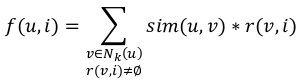
\includegraphics[width=0.4\textwidth]{images/knn_user}

 	 \subsubsection{Basado en item}
 	 	Se recomiendan al usuario los ítems que se parecen a ítems que le han gustado. Su función es muy similar a la del algoritmo k-NN con usuarios.\\
 	 	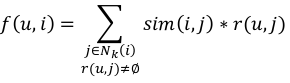
\includegraphics[width=0.4\textwidth]{images/knn_item}
 	 
 	 Normalmente, este algoritmo se utiliza con el número de vecinos igual al número total de ítems, es decir, que el vecindario de cada ítem son todos los demás existentes en el conjunto de datos. En cuanto a la función de similitud entre los usuarios o ítems, ésta se puede realizar mediante varios métodos, entre ellos destacan: 
 	 \begin{itemize}
 	 	\item \textbf{Coseno:} Mide el ángulo entre los vectores (ratings) década par de usuarios o ítems, de forma que son más similares aquellos cuyos vectores tienen la misma orientación. \\
 	 	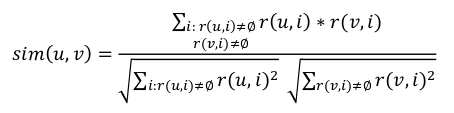
\includegraphics[width=0.7\textwidth]{images/coseno}

 	 	\item \textbf{Jaccard:} Dos usuarios o ítems son más similares cuanto más parecida sea la intersección a la unión de ambos, es decir, cuantos más ratings en común tengan, independientemente del valor de rating. \\
 	 	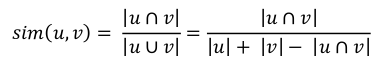
\includegraphics[width=0.5\textwidth]{images/jaccard}

 	 	\item \textbf{Pearson:} Equivalente a la similitud por coseno, pero cada rating se centra en la puntuación promedio del usuario (o ítem) correspondiente. Para este caso existen dos versiones dependiendo de la forma de calcular el módulo de v: por intersección, donde se suman los ratings de los ítems que tiene en común con u;y total, donde también se incluyen los ratings de aquellos que u desconoce. \\
 	 	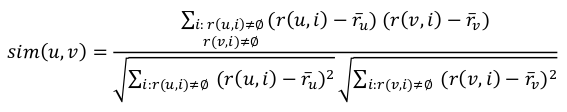
\includegraphics[width=0.8\textwidth]{images/pearson}

 	 \end{itemize}

 	\subsection{Slope One}
	El filtrado colaborativo es una técnica usada por los Sistemas de Recomendación para combinar las opiniones y pruebas de diferentes usuarios con el fin de obtener recomendaciones personalizadas. Hay al menos dos clases de filtrados colaborativos: las técnicas basadas en usuarios son derivadas de la medición de similitudes entre usuarios, mientras que las técnicas basadas en artículos comparan las valoraciones dadas por distintos usuarios. Slope One es una familia de algoritmos usados para el Filtrado Colaborativo introducida en Slope One Predictors for Online Rating-Based Collaborative Filtering por Daniel Lemire y Anna Maclachlan. Posiblemente, esta es la forma más simple de filtrado colaborativo basado en artículos. Su simplicidad la hace especialmente sencilla de implementar eficientemente mientras que su exactitud está a la par de algoritmos más complejos y costosos.
 	
 	\subsection{Factorización de matrices}
 		A los gustos de los usuarios y las características de los ítems subyace un espacio no visible que realmente determina por qué les gustan los ítems. Hay formalismos matemáticos que nos permiten hacer aflorar este tipo de espacio latente como unas cuantas dimensiones reducidas, sin tener que concretar qué son realmente esas dimensiones, y pudiendo sin embargo generar recomendaciones operando con ellas. La idea es representar tanto los ítems como los usuarios como vectores en un espacio de factores latentes, con una coordenada por factor que representa el grado de afinidad del usuario (o del ítem) hacia ese factor.Este efecto se puede realizar mediante la factorización de matrices representada en la figura~\ref{fig: matrix factorization}, descomponiendo la matriz original de ratings en un producto de varias matrices, dos o tres dependiendo del algoritmo, obteniendo siempre una primera matriz de usuarios por factores y una última de factores por ítems.

 		\begin{figure}[h!]
		 \centering
		 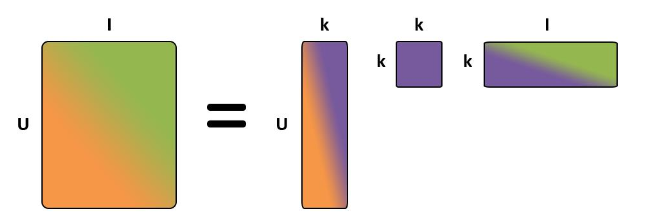
\includegraphics[width=12cm]{./images/matrix_fact}
		 \caption{Descomposición de la matrix en el producto de otras tres}
		 \label{fig: matrix factorization}
		\end{figure}

 		De esta forma, se obtienen k factores latentes que establecen un espacio de características común, tanto para los usuarios como para los ítems, permitiendo la comparación directa entre ellos.Así, un usuario da ratings de acuerdo a sus factores latentes y a los factores latentes del ítem.
 		A partir de aquí se ha desarrollado en el área gran cantidad de algoritmos para obtener la factorización de matrices, entre los que destacamos los siguientes:

 		\textbf{pLSA(probabilistic Latent Semantic Analysis):} Divide la matriz de ratings en dos, usuarios por factores y factores por ítems, de forma que su función de ránking equivale a la probabilidad de que el usuario puntúe al ítem según el espacio de factores latentes.\\
 		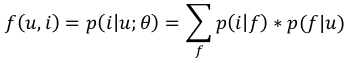
\includegraphics[width=0.5\textwidth]{images/plsa}

		\textbf{SVD(Singular Value Decomposition):} La factorización de la matriz de ratings genera tres matrices, para lo que se tiene en cuenta todos los ratings, asignándoles un cero a aquellos no conocidos. Se obtienen los vectores de usuario e ítem mediante el producto de las matrices obtenidas según la fórmula que se indica a continuación, de forma que su función de ránking consiste en la multiplicación de los vectores de usuario e ítem,centrado en la media del usuario.\\
		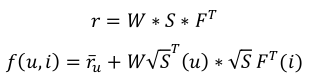
\includegraphics[width=0.5\textwidth]{images/svd}

		\textbf{SVDN(SVD no-empty entries):} Variante del anterior algoritmo en la que se obtienen dos matrices en lugar de tres,se tiene en cuenta únicamente los ratings conocidos, y su función de ránking no se centra en la media del usuario.\\
		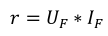
\includegraphics[width=0.2\textwidth]{images/svdn1}

		En este caso, entonces, el cálculo de dicha función es más inmediato, ya que los vectores de usuario e ítem se corresponden con la fila de la primera matriz y la columna de la segunda respectivamente, por lo que únicamente se multiplican la fila por la columna correspondiente.\\
		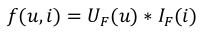
\includegraphics[width=0.4\textwidth]{images/svdn2}

		\textbf{HSVD(SVD with Hypergraph transformation):} Este método está dirigido a la recomendación de ítems a usuarios nuevos en el sistema, es decir, con poca actividad en el entrenamiento. Por ello, el primer paso del algoritmo consiste en dividir la matriz de ratings en tres: ratings de los usuarios que no están en test, ratings conocidos (de entrenamiento) de los usuarios que están en test, y ratings desconocidos de los usuarios que están en test (lo que se recomendará).

		\textbf{ASVD(Assymetric SVD):} Se trata de la versión asimétrica de SVD, que solo usa la tercera matriz de la descomposición para realizar las recomendaciones.Sigue exactamente los mismos pasos que HSVD, con la diferencia de que no se binariza la matriz de ratings de los usuarios viejos, sino que se utiliza la original con los ratings numéricos.

		\subsection{Basados en contenido}
		Este grupo de algoritmos se basa en la utilización de la descripción o características de cada ítem para realizar sugerencias sin utilizar información de otros usuarios para generar la recomendación. Destacan los algoritmos Rocchio y la implementación del k-NN para este tipo de sistemas de recomendación.
.
		\textbf{Rocchio:} Se basa en el cálculo de centroides para cada usuario, de forma que se obtenga un vector representante para cada uno. Estas clases se corresponderán con las características de los ítems, por ejemplo, en Twitter, las palabras clave del contenido de los tweets. De esta forma, se obtiene para cada usuario un centroide que representa su relación con cada característica. La fórmula para el cálculo de los centroides es la siguiente:\\
		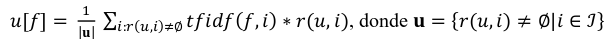
\includegraphics[width=\textwidth]{images/rocchio}
		Una vez se dispone de los centroides, el cálculo de la similitud de los usuarios con cada uno de los ítems se realiza mediante cualquiera de los métodos anteriormente descritos. 

		\textbf{k-NN (ítems):} Para la implementación del k-NN, la estructura de este algoritmo es idéntica a la de filtrado colaborativo del mismo nombre, su única diferencia radica en la forma de calcular la similitud entre los ítems.\\
		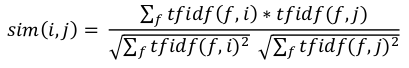
\includegraphics[width=0.5\textwidth]{images/knn_items}

		\subsection{Algoritmos no personalizados}
		Estos algoritmos recomiendan items sin conocer ningún dato del usuario, de forma impersonal como su propio nombre indica. 

		\textbf{Popularidad:} Recomienda los ítems por orden de popularidad y, por tanto, da exactamente el mismo ránking a cada uno de los usuarios. Por popularidad de un ítem se entiende el número de usuarios que han interactuado con el ítem en el sistema. Este método puede parecer trivial, pero es sin embargo uno de los más extendidos en escenarios reales.

		\textbf{Random:} Recomienda ítems de manera aleatoria a cada usuario y su precisión está relacionada con la densidad del conjunto de datos. La efectividad de la recomendación aleatoria, medida con una cierta métrica, se puede interpretar como la esperanza del valor de la métrica sobre el conjunto de datos en el que se aplica. \cite{11}

 \section{Bases de datos orientadas a grafos}
	Las bases de datos relacionales han existido por muchas décadas y son la tecnología de base de datos de elección para la mayoría de almacenamientos intensivos de datos y aplicaciones de obtención de datos. La obtención generalmente se logra mediante SQL, un lenguaje declarativo de consultas. Los sistemas de bases de datos relacionales son generalmente eficientes a menos que la información contenga muchas relaciones que requieren la unión de tablas grandes. Recientemente ha habido mucho interés en los almacenes de datos que no utilizan SQL exclusivamente, el llamado movimiento NoSQL. Ejemplos de ello son BigTable de Google y Cassandra de Facebook. \cite{7}

	Los modelos de bases de datos orientados a grafos se pueden caracterizar como aquellos en los que las estructuras de datos para el esquema y los casos se modelan en forma de grafos o generalizaciones de ellos, y la manipulación de datos se expresa mediante operaciones orientadas a grafos. Estos modelos nacieron en los años ochenta y principios de los noventa en paralelo a los modelos orientados a objetos y su influencia se desvaneció poco a poco con la aparición de otros modelos de bases de datos, en particular la geográfica, espacial, semi-estructurada y XML.

	Recientemente, la necesidad de gestionar la información con naturaleza inherente de un grafo ha hecho volver la relevancia de la zona. De hecho, una nueva ola de aplicaciones para bases de datos de grafos surgió con el desarrollo de las redes grandes (por ejemplo, Web, sistemas geográficos, transporte, teléfonos), y familias de redes generadas gracias a la automatización del proceso de recopilación de datos (por ejemplo, redes sociales y biológicas (incluyendo redes metabólicas, redes de interacción entre proteínas, grafos de estructuras químicas, clústers de genes, y mapas genéticos. Los grafos son realmente una de las más útiles estructuras para modelar objetos e interacciones.\cite{8}

	\subsection{Características}
		No hay índices clásicos en las bases de datos basadas en grafos. Por el contrario, cada objeto almacenado es representado por nodos (entidades) y aristas (relaciones). Un nodo es un registro único que tiene al menos una propiedad. Las aristas definen las relaciones entre los nodos y los nodos y sus relaciones tienen a su vez predefinidas conjuntamente propiedades. Los nodos pueden tener múltiples aristas que definen los diferentes tipos de relaciones que tienen con otros nodos.

		Las consultas en las bases de datos orientadas a grafos están diseñadas para empezar en un nodo específico y explorar sus relaciones con otros nodos. Un ejemplo podría ser: ¿Qué libros están leyendo mis amigos que yo aún no haya leído? Es por eso que este tipo de bases de datos están frecuentemente asociadas con motores de recomendación que se usan con frecuencia en aplicaciones sociales y de comercio electrónico.

		A medida que las búsquedas se van haciendo más complejas, el tiempo de procesamiento va aumentando. Es por eso que las bases de datos basadas en grafos aprenden e indexan las relaciones más comunes con el objetivo de acelerar el tiempo de búsqueda. 
		\subsubsection{Ventajas}
		\begin{itemize}
		 \item Rapidez para conectar datos. En las bases de datos relacionales, el frecuente uso de joins hace que las búsquedas sean lentas.
		 \item Sencillez de las consultas.
		 \item Rapidez en el manejo de consultas complejas que implican múltiples niveles de datos relacionados.
		\end{itemize}
		\subsubsection{Desventajas}
		\begin{itemize}
		 \item La búsqueda de nodos en diferentes máquinas puede ralentizar el proceso drásticamente.
		 \item Requiere un cambio conceptual para los desarrolladores, por lo que implica una curva de aprendizaje.
		\end{itemize}\cite{9}


 \section{Application Programming Interface (API)}
 	Una API (siglas de ‘Application Programming Interface’) es un conjunto de reglas (código) y especificaciones que las aplicaciones pueden seguir para comunicarse entre ellas: sirviendo de interfaz entre programas diferentes de la misma manera en que la interfaz de usuario facilita la interacción humano-software.

	Las API pueden servir para comunicarse con el sistema operativo (WinAPI), con bases de datos (DBMS) o con protocolos de comunicaciones (Jabber/XMPP). En los últimos años, por supuesto, se han sumado múltiples redes sociales (Twitter, Facebook, Youtube, Flickr, LinkedIn, etc) y otras plataformas online (Google Maps, WordPress…), lo que ha convertido el social media marketing es algo más sencillo, más rastreable y, por tanto, más rentable.

	Las API son valiosas, ante todo, porque \emph{permiten hacer uso de funciones ya existentes en otro software} (o de la infraestructura ya existente en otras plataformas) para no estar reinventando lo ya existente constantemente, reutilizando así componentes de software (código) cuyo funcionamiento ha sido probado y determinará una parte del nuevo proyecto. En el caso de herramientas propietarias (es decir, que no sean de código abierto), son un modo de hacer saber a los programadores de otras aplicaciones cómo incorporar una funcionalidad concreta sin por ello tener que proporcionar información acerca de cómo se realiza internamente el proceso. \cite{3}

	Eso es cierto incluso para los programas de código abierto. ¿Quién tiene el tiempo para revisar todo el código de la aplicación de otra persona, el cual puede ser terriblemente desordenado, sólo para usar una función? Las API simplifican todo al limitar el acceso fuera de programa a un conjunto específico de características, a menudo suficientes. Se definen claramente exactamente cómo un programa que va a interactuar con el resto del software, ahorrar recursos y enredos legales potencialmente desagradables en el camino. \cite{10}

  \chapter{Análisis general del proyecto}
	Para el desarrollo del sistema en su totalidad, se realizó el siguiente análisis general que define en su totalidad al proyecto.

	\section{Características}
		Para que el sistema se considere que ha cumplido con los objetivos planteados debe contar con las siguientes características dentro de su funcionalidad.
		\begin{itemize}			
			\item El sistema permitirá la búsqueda de platillos.
			\item El sistema permitirá obtener recomendaciones de acuerdo a las características de un platillo.
			\item El sistema obtendrá información de la interacción del usuario a través de evaluaciones explícitas, y conteo de clics implícitos hacia los platillos para obtener recomendaciones personalizadas para dicho usuario.
			\item El sistema permitirá el registro de usuarios finales.
			\item El sistema generará recomendaciones de platillos de acuerdo a la información proporcionada de los usuarios registrados, con base en sus evaluaciones y características.
			\item El sistema permitirá al usuario agregar nuevos platillos que haya consumido en cierto restaurante.
			\item El sistema permitirá al usuario administrar los platillos que agregó. 
		\end{itemize}

	\section{Restricciones}
		Debido a diferentes aspectos, el sistema contará con las siguientes restricciones.
		\begin{itemize}
			\item El sistema se verá limitado a las tecnologías empleadas para su desarrollo.
			\item El sistema puede verse limitado debido a la dependencia de fuentes de información externas.
			\item El sistema puede verse limitado en desempeño y precisión debido a la cantidad de información almacenada y a la complejidad del problema a resolver.
		\end{itemize} 

	\section{Estudio de factibilidad}
Después de definir la problemática presente y presentar la propuesta de solución, es  pertinente realizar un estudio de factibilidad para determinar la infraestructura tecnológica y la capacidad técnica que implica la implementación de la API en cuestión. Este análisis permite determinar las posibilidades de diseñar a API propuesta y su puesta en marcha. 
\\\\
A continuación se describen los aspectos que se toman en cuenta para este análisis.
\subsection{Factibilidad técnica }
Consiste en realizar una evaluación de la tecnología existente; este estudio está destinado a recolectar información sobre los componentes tecnológicos que posee este equipo de desarrollo y la posibilidad de utilizarlos en el desarrollo e implementación de este trabajo y de ser necesario, los requerimientos tecnológicos que deben ser adquiridos su desarrollo e implementación. 
\\\\
Hardware 
\\\\
Para el desarrollo de la API se cuentan con 3 computadoras personales, las cuales cuentan 
con las siguientes características:
\begin{itemize}
 \item MacBook Pro 13: 4 GB DDR3 RAM, Procesador Intel i5 a 2.5 GHz. S.O
 \item HP 8 GB DDR3 RAM, Procesador A10 2.1 GHz. S.O. Ubuntu 14.04.
 \item Acer 8 GB DDR3 RAM Procesador AMD A6 2.0 GHz. Ubuntu 14.04LTS.
\end{itemize}


% Los módulos desarrollados para la primera parte del Trabajo Terminal serán expuestos de 
% manera local, accediendo a ellos a través de una red local. Para la segunda entrega del 
% Trabajo Terminal se tiene planeado exponerlos en un servidor, para lo cual se contará un 
% servicio de hosting. No se incluirá en este documento la opción elegida para el hosting ni el 
% costo del mismo, ya que no se sabe con exactitud cual se elegirá, a pesar de que se han 
% tomado en cuenta varios, no se ha llegado a una decisión.
\newpage
Software  
\\\\
Actualmente el desarrollo de este tipo de proyectos cuenta con la ventaja de existir múltiples tecnologías sobre las cuales es posible desarrollarlo. Por mencionar algunas, el proyecto está pensado para ser desarrollado sobre tecnologías como las listadas a continuación.
\begin{itemize}
\item Java
\item Neo4j
\item Hibernate
\item JavaScript
\item HTML
\item Boostrap
\item Spring
\item Maven
\end{itemize}
Estas tecnologías son necesarias para el desarrollo de esta API, cada una cumple con un objetivo específico pero no son indispensables ya que se encuentran muchos otras disponibles con las cuales es posible realizar el desarrollo del proyecto. Para un mayor análisis de opciones disponibles actualmente, revise el apartado de \emph{Tecnologías}.
\\\\
Costos 
\\\\
Los costos que generará el desarrollo de este proyecto se calcularon de la siguiente manera: 
\begin{itemize}
\item El manejo roles se repartió en el equipo, es decir, cada miembro del equipo cumplió las tareas de analizar, diseñar y desarrollar.  
\item Nos basamos en un sueldo promedio al cual aspiran estudiantes de la carrera de 
Ing. en Sistemas Computacionales, que es de \$78
\end{itemize}
Después de aclarar lo siguiente, los costos operacionales (mano de obra) se calcularon así:
\begin{itemize}
\item 3 personas que desarrollan diferentes actividades 
\item Cada uno gana \$78 la hora desarrollando el proyecto
\item Se toma en cuenta que se trabajan 5 días de la semana 5 horas cada uno de ellos, así: 
\end{itemize}
(\$78) * (5 hrs) * (250 dias) * (3 personas) = \$292,500
 
El precio estimado de este sistema es de \$292,500 MXN solamente tomando en cuenta la mano de obra, sin contemplar nuevos equipos, reuniones, transportes, comida y horas extras. En las siguientes páginas se procede a describir el análisis técnico del proyecto.
\newpage

  \section{Metodología}
	\subsection{Descripción}
	  Para ese proyecto se plantea usar una metodología de prototipado evolutivo, que se caracteriza por que en su modelo de trabajo un prototipo es construido, probado y finalmente reconstruido las veces que sea necesario hasta que un prototipo aceptable es finalmente alcanzado del cual el sistema completo o producto puede ser totalmente desarrollado.

	  Este modelo funciona bien en escenarios donde no se conocen por completo los requerimientos. Así los prototipos, modelos de software con una funcionalidad limitada, permiten al usuario evaluar los propósitos del desarrollador y probarlos antes de su implementación. También ayuda a entender los requerimientos específicos del usuario y que no pudieron haber sido considerados por el desarrollador durante el diseño del sistema.

	\subsection{Prototipos esperados}
	  De acuerdo al modelo de desarrollo elegido, se han establecido los siguientes prototipos y sus alcances que se pueden observar en el cuadro~\ref{table:prototipos}

	  \begin{table}[h]
	  \begin{center}
	  \begin{tabular}{ | c | c | }
	    \toprule
	    	\textbf{Versión} & \textbf{Alcance} \\
	    \midrule
	    	Prototipo 1 & Obtener y abstraer los datos a utilizar\\
	    \midrule
	    	Prototipo 2 & Visualizar los datos en recomendaciones por contenido\\
	    \midrule
	    	Prototipo 3 & Obtener recomendaciones para diversos fines (sistemas híbridos) \\
	    \midrule
	    	Prototipo 4 & Desarrollar un sistema híbrido de recomendación para platillos y restaurantes. \\
	    \bottomrule
		\end{tabular}
	  \caption{Cuadro de prototipos esperados}
  	  \label{table:prototipos}
  	\end{center}
	\end{table}


  \section {Descripción y módulos del sistema}
% \section{¿Para qué sirve el sistema?}

  \subsection{Arquitectura general}
    \paragraph{Para desarrollar un sistema de recomendacion se han planteado los siguientes módulos funcionales de la API, el cual será utilizado por el desarrollador final para que, en conjunto con su aplicación final realice la integración de las funciones disponibles en el API junto al sistema de recomendación final. Esto se puede denotar en el siguiente diagrama.}

\newpage
    \begin{landscape}
      \begin{figure}[h!]
      \centering
      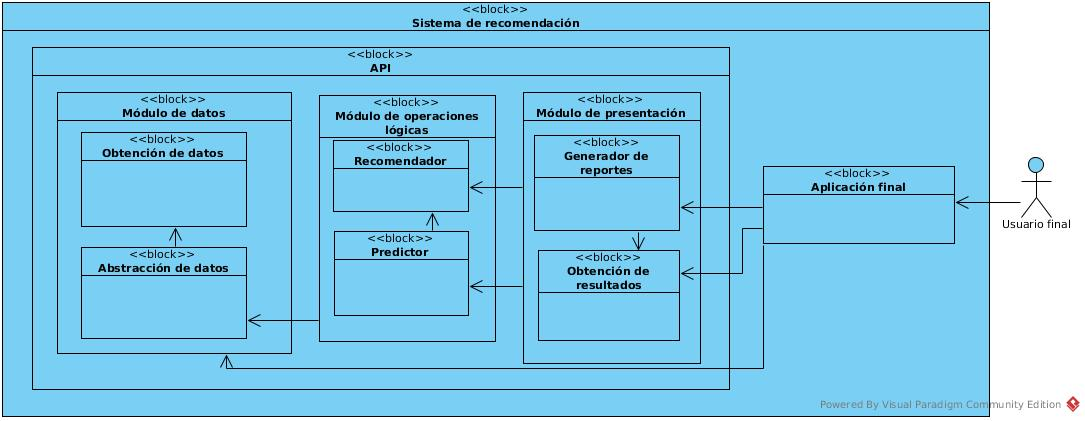
\includegraphics[width=22.5cm,height=12cm]{./images/architecture_diagram.jpg}
      \caption{Diagrama general del sistema}
    \end{figure}
    \end{landscape}
  \newpage

\paragraph{Cómo se apreciar en el diagrama, el sistema se encuentra dividido en tres módulos básicos además de la aplicación final que hace uso de los módulos de la API.}
    \begin{itemize}
    \item Módulo de datos
    \item Módulo de operaciones lógicas
    \item Módulo de presentación
    \item Caso de estudio ó aplicación final
  \end{itemize}

\subsection{Módulos de la API}
  \subsubsection{Módulo de abstracción de datos}
    \paragraph{Este módulo es el encargado de la obtención de datos para su adecuada manipulación dentro de los objetivos del sistema, es decir, permitirá el manejo de los datos estandarizandolos a un modelo de datos base que permitirá tener la funcionalidad del sistema de recomendación de manera adecuada. }
    \paragraph{Se presenta como un módulo conformado por diferentes interfaces de conexión para fuentes de datos, como pueden ser ficheros de texto o la conexión a un gestor de base de datos. Tiene una interacción directa con el módulo de operaciones lógicas dentro del sistema.}

  \subsubsection{Módulo de operaciones lógicas}
    \paragraph{El módulo de operaciones lógicas permitirá, haciendo uso de la información almacenada, obtener recomendaciones y predicciones de los diferentes artículos deacuerdo a diferentes clasificaciones con base en los principales tipos de recomendacion existentes: basados en contenido y colaborativos. Cabe destacar, la constante operación de este módulo para el aprendizaje y mejora constante de las recomendaciones.}

  \subsubsection{Módulo de presentación}
    \paragraph{Haciendo uso del módulo de operaciones lógicas, este módulo pretende brindar la funcionalidad de mostrar en forma de reportes tabulares, los resultados obtenidos de la recomendación al ser integrado en la aplicación final.}

\subsection{Aplicación final}
  \subsubsection{Definición}
    \paragraph{En este caso, la aplicación final hará uso de las funciones proporcionadas por los distintos módulos que conforman la API para obtener recomendaciones de los datos que pertenezcan a su caso de estudio. Interactúa directamente con el módulo de abstraccion de datos y con el módulo de presentación para hacer uso de la funcionalidad permitida por el API. En este caso, la aplicación final se verá reflejada en un sistema web que permita denotar la funcionalidad de la API para un conjunto de datos de platillos y restaurantes.}
  \section{Análisis y gestión de riesgos}
  \subsection{Definición y clasificación}
    El riesgo siempre implica una incertidumbre y una pérdida potencial, al identificar estos riesgos podemos determinar su naturaleza en tres tipos diferentes para este proyecto:
    \begin{itemize}
      \item Riesgos del proyecto
      \item Riesgos técnicos
      \item Riesgos de negocio
    \end{itemize}
    Así mismo, es necesario clasificar los riesgos existentes de acuerdo  a la probabilidad de que éstos ocurran. Para lo cual se utilizará los siguientes valores por convención.
    \begin{itemize}
      \item Muy bajo ( < 10\% )
      \item Bajo ( 10 - 25\% )
      \item Moderado (25 - 50\% )
      \item Alto (50 - 75\% )
      \item Muy Alto ( > 75\% )
    \end{itemize}
    Así mismo, todos los riegos depen categorizarse deacuero al impacto que pueden causar en el sistema en las siguientes categorías: Insignificante, Tolerable, Serio, Catastrófico; los planes de contingencia suelen ser desarrollados para aquellos riegos con probabilidad de moderada a muy alta y con un impacto serio o castastrófico.
    A continuación se plantean los riesgos identificados para el sistema general a lo largo del desarrollo del mismo y sus respectivos planes de acción.
    \newpage
    \begin{table}[b!]
    \centering
      \begin{tabular}{|p{3cm}|lllll}
        \hline
        \multicolumn{5}{|c|}{{\bf Tabla de Riesgos}} \\ 
        \hline
          \multicolumn{1}{|p{3cm}|}{{\bf Descripcion}} & 
          \multicolumn{1}{p{2cm}|}{{\bf Tipo de Riesgo}} & 
          \multicolumn{1}{p{2cm}|}{{\bf Valoración}} & 
          \multicolumn{1}{p{2cm}|}{{\bf Porcentaje}} & 
          \multicolumn{1}{p{5cm}|}{{\bf Plan de acción}} \\ 
        \hline
          \multicolumn{1}{|p{3cm}|}{Falta de presupuesto} & 
          \multicolumn{1}{p{2cm}|}{Proyecto} & 
          \multicolumn{1}{p{2cm}|}{Serio} & 
          \multicolumn{1}{p{2cm}|}{25\%} & 
          \multicolumn{1}{p{5cm}|}{Buscar un proceso de incubación en empresas como Apache, Eclipse y migrar la plataforma a servicios de hosting gratuitos como Heroku u Openshift.} \\ 
        \hline
          \multicolumn{1}{|p{3cm}|}{Falta por razones personales de miembros del equipo} & 
          \multicolumn{1}{p{2cm}|}{Proyecto} &
          \multicolumn{1}{p{2cm}|}{Serio} & 
          \multicolumn{1}{p{2cm}|}{25\%} & 
          \multicolumn{1}{p{5cm}|}{Rediseñar y adaptar las tareas con nuevos integrantes y habilitar forma de trabajo remota considerando fines de semana.} \\ 
        \hline
          \multicolumn{1}{|p{3cm}|}{Necesidad de escalabilidad de la plataforma} & 
          \multicolumn{1}{p{2cm}|}{Técnico} & 
          \multicolumn{1}{p{2cm}|}{Serio} & 
          \multicolumn{1}{p{2cm}|}{10\%} & 
          \multicolumn{1}{p{5cm}|}{Definir el tipo de escalabilidad a usar dependiendo los recursos monetarios existentes.} \\ 
        \hline
          %\multicolumn{1}{|p{3cm}|}{Ataques de Denegación de Servicios (DoS)} & 
          %\multicolumn{1}{p{2cm}|}{Técnico} & 
          %\multicolumn{1}{p{2cm}|}{Tolerable} & 
          %\multicolumn{1}{p{2cm}|}{10\%} & 
          %\multicolumn{1}{p{5cm}|}{} \\ 
        %\hline
      \end{tabular}
      \caption{Analisis de Riesgos}
      \label{Analisis de riesgos}
    \end{table}
    \clearpage
  \section{Tecnologías}
Para el desarrollo del proyecto se propone utilizar las siguientes tecnologías que permitirán lograr los objetivos propuestos en el sistema. Las ventajas que representan para el desarrollo son descritas a continuación.
\vspace{-15mm}
	\begin{table}[b!]
    \centering
      \begin{tabular}{|p{2cm}|ll}
        \hline
        \multicolumn{2}{|c|}{{\bf Cuadro comparativo de tecnologías}} \\ 
        \hline
          \multicolumn{1}{|p{4cm}|}{{\bf Nombre}} & 
		  \multicolumn{1}{p{10cm}|}{{\bf Características}}\\

        \hline
          \multicolumn{1}{|p{5cm}|}{
\includegraphics[width=0.3\textwidth]{images/neo4j}} & 
          \multicolumn{2}{p{10cm}|}{\begin{itemize}
          \vspace{-15mm}
        \item Es una base de datos open-source,esta escrita en java.
        \item Permite realizar transacciones ACID.
        \item Manera su propio lenguaje de query , Cypher.
        \item Puede contener billiones de nodos y relaciones.
        \item Rápido recorriendo relaciones, este tipo de queries se conoce como transversals
        \item Las escrituras se pueden realizar en cualquier instancia del clúster.
        \item Multilenguaje, proporciona una Api Rest pudiendo utilizarse desde cualquier lenguaje.
      \end{itemize}} \\
         
        \hline
          \multicolumn{1}{|p{5cm}|}{
\includegraphics[width=0.3\textwidth]{images/InfiniteGraph}} & 
          \multicolumn{1}{p{10cm}|}{
          \begin{itemize}
          \vspace{-7mm}
        \item Posee almacenamiento en la nube.
        \item Apoyo de consultas en paralelo.
        \item Precios felixibles y opciones de licencia.
        \item Totalmente transaccional y multi-hilo,
      \end{itemize}} \\ 
        \hline
          \multicolumn{1}{|p{3cm}|}{
\includegraphics[width=0.3\textwidth]{images/InfoGrid}} & 
          \multicolumn{1}{p{10cm}|}{
          \begin{itemize}
          \vspace{-10mm}
        \item Recorrido Gráfico y consultas de tipo relacional.
        \item Indexación personalizable.
        \item Gestión de almacenamiento personalizable.
      \end{itemize}}\\ 
         \hline
        %\hline
      \end{tabular}
      \caption{Cuadro comparativo de gestores de bases de datos orientadas a grafos}
      \label{table:bd orientadas a grafos}
    \end{table}
\newpage
\begin{table}[b!]
    \centering
      \begin{tabular}{|p{1cm}|l}
        \hline
        \multicolumn{2}{|c|}{{\bf Cuadro comparativo de tecnologías}} \\ 
        \hline
          \multicolumn{1}{|p{4cm}|}{{\bf Nombre}} & 
		  \multicolumn{1}{p{10cm}|}{{\bf Características}}\\
		 \hline
          \multicolumn{1}{|p{5cm}|}{
\includegraphics[width=0.3\textwidth]{images/bootstrap}} & 
          \multicolumn{1}{p{10cm}|}{\begin{itemize} 
       \vspace{-20mm}
          \item Es un framework o conjunto de herramientas de software libre para diseño de sitios y aplicaciones web. 
        \item Contiene plantillas de diseño con tipografía, formularios, botones, cuadros, menús de navegación y otros elementos de diseño basado en HTML y CSS, así como, extensiones de JavaScript opcionales adicionales.
        \item Es compatible con la mayoría de los navegadores web.
        \item Bootstrap es de código abierto y está disponible en GitHub. 
        \item Desde la versión 2.0 también soporta diseños sensibles. Esto significa que el diseño gráfico de la página se ajusta dinámicamente, tomando en cuenta las características del dispositivo usado (Computadoras, tabletas, teléfonos móviles).
      \end{itemize}} \\
         
        \hline
          \multicolumn{1}{|p{5cm}|}{
\includegraphics[width=0.3\textwidth]{images/foundation}} & 
          \multicolumn{1}{p{10cm}|}{ 
          \begin{itemize}
                 \vspace{-20mm}
          \setlist[itemize]{noitemsep, topsep=0pt}  
          	\item No tiene que agregar clases de responder o lograr cierto estilo.
			\item Muchos prefieren Foundation, ya que ofrece más flexibilidad.
			\item Fácil navegación de su sitio a otro sitio.
            \item Tablas de precios,diseñado para mostrar los precios de un producto a base de suscripción
            \item Las páginas web se ajustan a diferentes dispositivos.
         \end{itemize}}\\ 
        \hline
        %\hline
      \end{tabular}
      \caption{Cuadro de tecnologías para diseño Web}
      \label{table:tecnologias web}
    \end{table}


  \chapter{Prototipo 1: Obtener y abstraer los datos a utilizar}
  \section{Análisis}
    \subsection{Objetivo}
      Crear el módulo de conexión de datos apropiado para el manejo de la información de acuerdo a un modelo de datos propuesto diseñado por el equipo de trabajo.

    \subsection{Características}
      \begin{itemize}
        \item El modelo de datos propuesto deberá satisfacer las necesidades para trabajar con diferentes artículos y la interacción con sus usuarios.
        \item El sistema deberá permitir la conexión a la fuente de datos que corresponda con el modelo propuesto.
        \item El sistema deberá ser capaz de realizar operaciones sobre los datos de la fuente para el correcto funcionamiento de los procesos lógicos del sistema.
      \end{itemize}

    \subsection{Restricciones}
      \begin{itemize}
        \item El sistema se verá limitado por el lenguaje de desarrollo Java.
        \item Para el caso de estudio, el sistema operará con el gestor de base de datos propio de Neo4j. 
      \end{itemize}

  \section{Diseño}
    \subsection{Modelo de datos}
      Para la API, el problema fundamental recae en que las recomendaciones pueden ser utilizadas para diversos casos de estudio, buscando una generalización de las características mínimas requeridas para realizar recomendaciones se plantea un modelo de datos utilizando tres principales entidades: Usuarios, Artículos a recomendar, y Categorías como características que permitan clasificar los diferentes artículos. La información que será guardada y posteriormente consultada por otros módulos del sistema seguirá un esquema propuesto por el equipo de trabajo, éste recopila la estructura de evaluaciones básicas generadas en prácticamente cualquier tipo de artículos, películas, platillos, libros, entre otros como se puede apreciar en la figura~\ref{fig:general_model}.

            \begin{figure}[h!]
            \centering
            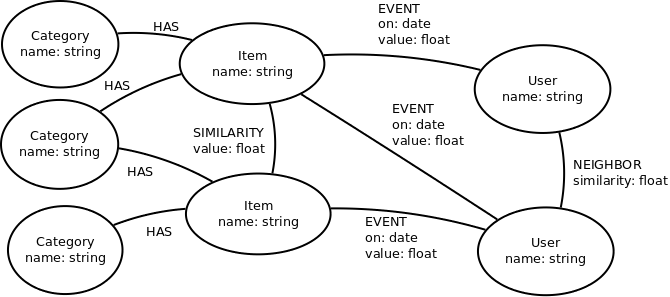
\includegraphics[width=16cm]{./images/general_data_model.png}
            \caption{Modelo general necesario para el manejo de la información}
            \label{fig:general_model}
          \end{figure}

      
  \section{Resultados}
    Para la aplicación cliente correspondiente al caso de estudio de recomendación de platillos, el sistema tendrá un modelo de datos que parte del modelo general mínimo necesario para trabajar la información añadiendo información relevante sobre el caso de estudio que recae en platillos como artículos a recomendar. Considerando al final las siguientes entidades.
      \begin{itemize}
        \item Platillos
        \item Usuarios
        \item Restaurantes
        \item Categorías
      \end{itemize}

      La figura~\ref{fig:data model} muestra las entidades utilizadas en el sistema de recomendación de platillos así como las relaciones existentes entre las mismas. En éste los nodos del grafo corresponden a las entidades Usuario, Platillo, Restaurante y Categoría. Donde las relaciones entre ellos se describen de la siguiente manera: 
      \begin{itemize}
        \item Un platillo puede ser de una o más categorías.
        \item Un platillo puede ser servido en uno o más restaurantes
        \item Un usuario puede agregar un platillo
        \item Un usuario puede interactuar con un platillo a través de un conteo de clics.
        \item Un usuario puede evaluar qué tanto le gustó un platillo a través de un rating cuantitativo.
      \end{itemize} 

      \begin{landscape}
        \begin{figure}[h!]
          \centering
          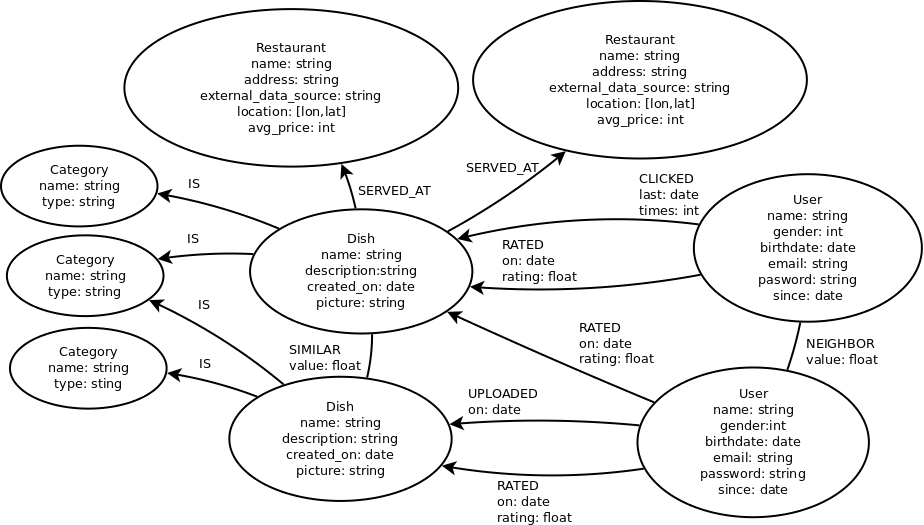
\includegraphics[width=22.5cm,height=12cm]{./images/sc_data_model.png}
          \caption{Modelo de datos propuesto para el caso de estudio}
          \label{fig:data model}
        \end{figure}
      \end{landscape}

    Utilizando el modelo propuesto por el equipo de trabajo, es posible generar datos de prueba con contenido de platillos así como proponer una serie de categorías que fungirán como características para clasificar los diferentes platillos. Las categorías propuestas se identifican por diferentes rubros como son: tipo de comida, sabor, ocasión, región, salud, temperatura, como podemos notarlas en el anexo~\ref{table:caracteristicas}.\cite{23,24}

    Como resultado de la implementación del modelo de datos para el sistema, se obtuvieron datos utilizando la técnica de web-scrapping para obtener información de platillos de prueba. La figura~\ref{fig:neo4j graph} muestra la siguiente representación gráfica del modelo utilizado en el caso de estudio. 
          \begin{figure}[h!]
            \centering
            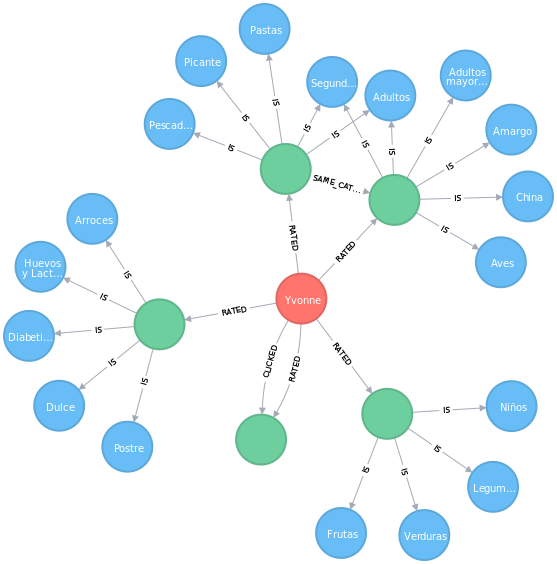
\includegraphics[width=12cm]{./images/graph}
            \caption{Modelo de datos implementado para el caso de estudio}
            \label{fig:neo4j graph}
          \end{figure}

  \chapter{Prototipo 2: Visualizar los datos en recomendaciones por contenido}
  \section{Análisis}
    \subsection{Objetivo}
      Visualizar recomendaciones bajo el filtrado por contenido de los platillos contenidos en el sistema. 

    \subsection{Características}
    \begin{itemize}
      \item El sistema permite al usuario visualizar los platillos.
      \item El sistema muestra recomendaciones de acuerdo a un solo platillo, para mostrar los que tienen una mayor similitud con éste.
      \item El sistema permite la interacción de usuarios no registrados para obtener recomendaciones personalizadas con base en los platillos que ha visualizado.
      \item La evaluación de similitud se logra a través de las características en común que tengan los platillos entre sí.
    \end{itemize}

    \subsection{Restricciones}
    \begin{itemize}
      \item El sistema se ve limitado a la cantidad y características de los platillos existentes actualmente.
      \item El usuario no registrado no podrá modificar o eliminar los platillos del sistema.
    \end{itemize}
  \newpage
  \section{Diseño}
    Para la implementación de las recomendaciones por contenido, se consideran las características que tienen en común. La cantidad de características que poseen en común es identificada por una evaluación de similitud. Dicha evaluación genera un conjunto de relaciones con las que es posible determinar los artículos que se parecen más entre sí y obtener los vecinos más cercanos a cada elemento. Así, para los platillos, las características a las que pertenecen, permiten crear una vecindad para cada nodo donde es posible obtener cuáles son los platillos vecinos que más se parecen entre sí.

    \subsection{Diagrama de clases}
    Implementando el comportamiento descrito anteriormente se generan las clases mostradas en la figura~\ref{fig: diagrama clases p2} que permiten obtener las recomendaciones por contenido. 
          \begin{figure}[h!]
          \centering
          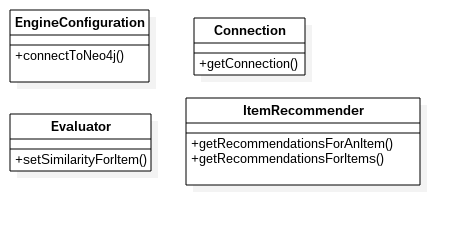
\includegraphics[width=12cm]{./images/p2_classes.png}
          \caption{Diagrama de clases del prototipo 2}
          \label{fig: diagrama clases p2}
        \end{figure}

    \subsection{Casos de uso}
    Integrando la funcionalidad planteada en las clases anteriores dentro de un sistema web que permita la interacción del usuario se plantean los siguientes casos de uso mostrados en la figura~\ref{fig:CU p2}
    \begin{figure}[h!]
      \centering
      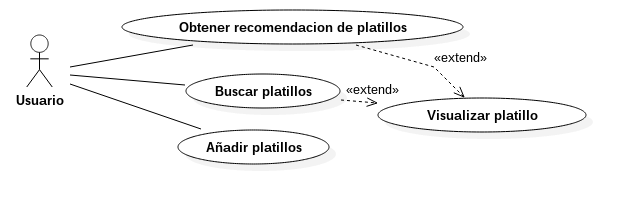
\includegraphics[width=16cm]{./images/prototipo2.png}
      \caption{Casos de uso del prototipo 2}
      \label{fig:CU p2}
    \end{figure}
    
    \paragraph{CU. Obtener recomendación de platillos\\} 
    \textbf{Descripción:} El usuario obtiene recomendaciones del sistema\\
    \textbf{Actores:} Usuario \\
    \textbf{Precondiciones:} Ninguna \\
    \textbf{Flujo normal}\\
    \begin{itemize}
      \item El sistema muestra información de platillos relevantes no personalizadas.
    \end{itemize}
    \textbf{Flujo alternativo}\\
    \begin{itemize}
      \item El sistema muestra recomendaciones personalizadas de acuerdo a interacciones previas del usuario.
    \end{itemize}

    \paragraph{CU. Buscar platillos\\}
    \textbf{Descripción:} El usuario utiliza el sistema de búsqueda para encontrar platillos relacionados.\\
    \textbf{Actores:} Usuario\\
    \textbf{Precondiciones:} Ninguna\\
    \textbf{Flujo normal}\\
    \begin{itemize}
      \item El usuario escribe su búsqueda en el sistema. 
      \item El sistema obtiene los platillos encontrados, así como platillos relacionados
      \item El sistema muestra los resultados al usuario
    \end{itemize}

    \paragraph{CU. Visualizar platillo\\}
    \textbf{Descripción:} El usuario visualiza la información descriptiva de un platillo\\
    \textbf{Actores:} Usuario\\
    \textbf{Precondiciones:} El usuario selecciona un platillo desde el CU. Obtener recomendación de platillos o desde el CU. Buscar platillos\\
    \textbf{Flujo normal}\\
    \begin{itemize}
      \item El usuario selecciona un platillo de la lista de resultados
      \item El sistema muestra la información descriptiva de ese platillo.
    \end{itemize}
    \newpage
    \paragraph{CU. Agregar platillo\\}
    \textbf{Descripción:} El usuario agrega un platillo en el sistema\\
    \textbf{Actores:} Usuario\\
    \textbf{Precondiciones:} Ninguna\\
    \textbf{Flujo normal}\\
    \begin{itemize}
      \item El sistema muestra el método de entrada para las características de los platillos
      \item El usuario introduce los parámetros necesarios para registrar el platillo. (Nombre, descripción y características que le describen)
      \item El sistema carga la información del platillo al sistema.
    \end{itemize}
    \textbf{Flujo alternativo}\\
    \begin{itemize}
      \item El sistema comprueba la validez de los datos, si no son correctos, se avisa al actor permitiendo que se corrijan. 
      \item Si el sistema no puede salvar la información del nuevo platillo, se notifica al usuario que el platillo no ha sido agregado.
    \end{itemize}
    
  \section{Resultados}
    Tras definir las acciones realizadas en el prototipo, se realiza el desarrollo del sistema Bonappettit, prototipo del sistema final que permite obtener recomendaciones con filtrado por contenido para usuarios no registrados en la plataforma. Esta plataforma se ve implementada en un sistema web cuyo estilo visual es posible de apreciar en la figura~\ref{fig: screenshot1 p2}\\
        \begin{figure}[h!]
          \centering
          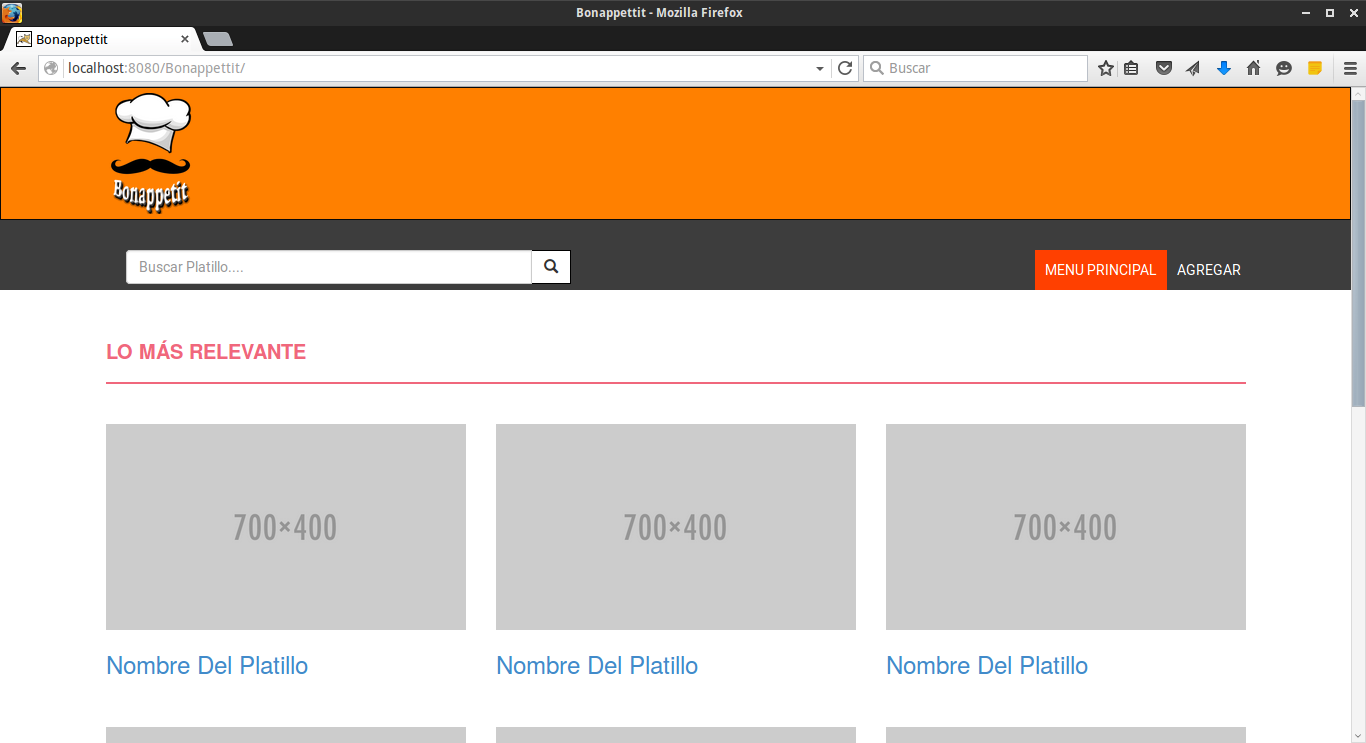
\includegraphics[width=16cm]{./images/bonappettit.png}
          \caption{Capturas de pantalla del sistema}
          \label{fig: screenshot1 p2}
        \end{figure}

    Así mismo, podemos denotar el resultado de las recomendaciones para un ítem en particular como prueba de la implementación del algoritmo k-NN implementado para reconocer la similitud entre los diversos platillos que se encuentran registrados en el sistema, como se describió en el diseño del prototipo. Debido a la ausencia de usuarios registrados en el sistema, y a la falta de información de restaurantes de una zona en particular, el prototipo se ve limitado a recomendar platillos de acuerdo a sus características por filtrado por contenido. Actualmente se cuenta con registro de 843 platillos dentro de la base de datos disponibles para hacer pruebas con las recomendaciones necesarias, se espera este número aumente con el tiempo. Por lo mismo, del modelo de datos propuesto para el caso de estudio en la figura~\ref{fig:data model}, para este prototipo se ve limitado al modelo observado en la figura~\ref{fig:p2 db} solo permitiendo la recomendación de platillos. Como prueba de su funcionamiento, la figura~\ref{fig:screenshot2 p2} muestra el resultado de la recomendación para la búsqueda de ensaladas, de acuerdo a las características denotadas por las características a las que pertenece el primer platillo encontrado. 

      \begin{figure}[h!]
          \centering
          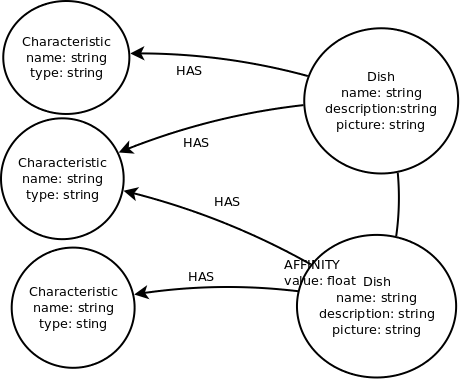
\includegraphics[width=16cm]{./images/p2_model}
          \caption{Modelo de datos con funcionalidad limitada para el prototipo 2}
          \label{fig:p2 db}
        \end{figure}

        \begin{figure}[h!]
          \centering
          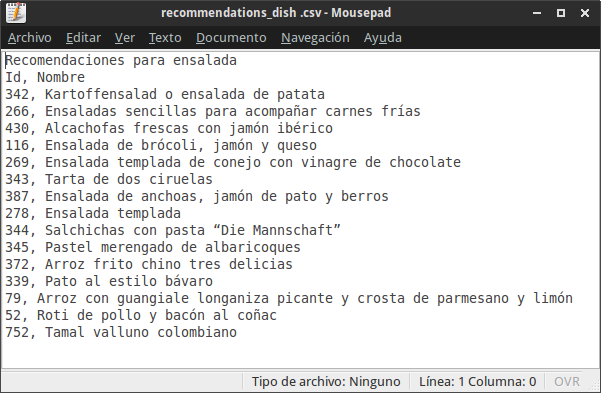
\includegraphics[width=16cm]{./images/recommendations_dish}
          \caption{Recomendación obtenida para la búsqueda de ensaladas}
          \label{fig:screenshot2 p2}
        \end{figure}
  \chapter{Prototipo 3: Obtener recomendaciones para diversos fines (sistemas híbridos)}
  \section{Análisis}
    \subsection{Objetivo}
      Generar las operaciones lógicas necesarias para realizar recomendaciones generalizadas para sistemas híbridos.

    \subsection{Características}
    \begin{itemize}
      \item El sistema proveerá las reglas, especificaciones y funciones necesarias para obtener recomendaciones de cualquier tipo de artículo que esté acorde al modelo propuesto.
      \item El sistema proveerá la funcionalidad de recomendaciones híbridas (basadas en contenido y colaborativas).
      \item El sistema proveerá los servicios necesarios para hacer posible la extensión de las funcionalidades desarrolladas.
    \end{itemize}

    \subsection{Restricciones}
    \begin{itemize}
      \item El sistema será capaz de obtener recomendaciones de artículos solo que empaten con el modelo propuesto. 
      \item El sistema será capaz de obtener recomendaciones de acuerdo a la funcionalidad desarrollada hasta el momento, siendo capaz de extender su funcionalidad a través de interfaces implementables.
    \end{itemize}

  \section{Diseño}
  Para la generalización de las recomendaciones sobre cualquier objeto acorde al modelo propuesto, se desarrollaron servicios basados en interfaces que permiten al desarrollador, utilizar la funcionalidad de la API, así como abstraer y modelar los objetos propios del sistema que desean desarrollar. 

  Para esto se utilizaron las interfaces Item, Characteristic y User, de las cuales las clases del dominio implementan para modelar cada uno de los comportamientos descritos para cada uno de los tipos de entidad identificados por las interfaces, permitiendo la obtención de los datos para el funcionamiento de la API y a su vez, la manipulación de los mismos en los procesos lógicos desarrollados en la API.

  Así mismo, para establecer las relaciones existentes entre estas entidades fue necesario establecer las interfaces Event, Neighbor y Affinity. Cada una de estas describe un comportamiento propio de las características de la relación. Como se puede ver en la figura~\ref{fig:p3_interfaces}, estas interfaces planteadas determinan el comportamiento de la API descrito en los párrafos posteriores, modelando las entidades y relaciones de la figura~\ref{fig:p3_general_model}

  \begin{landscape}
    \begin{figure}[h!]
      \centering
      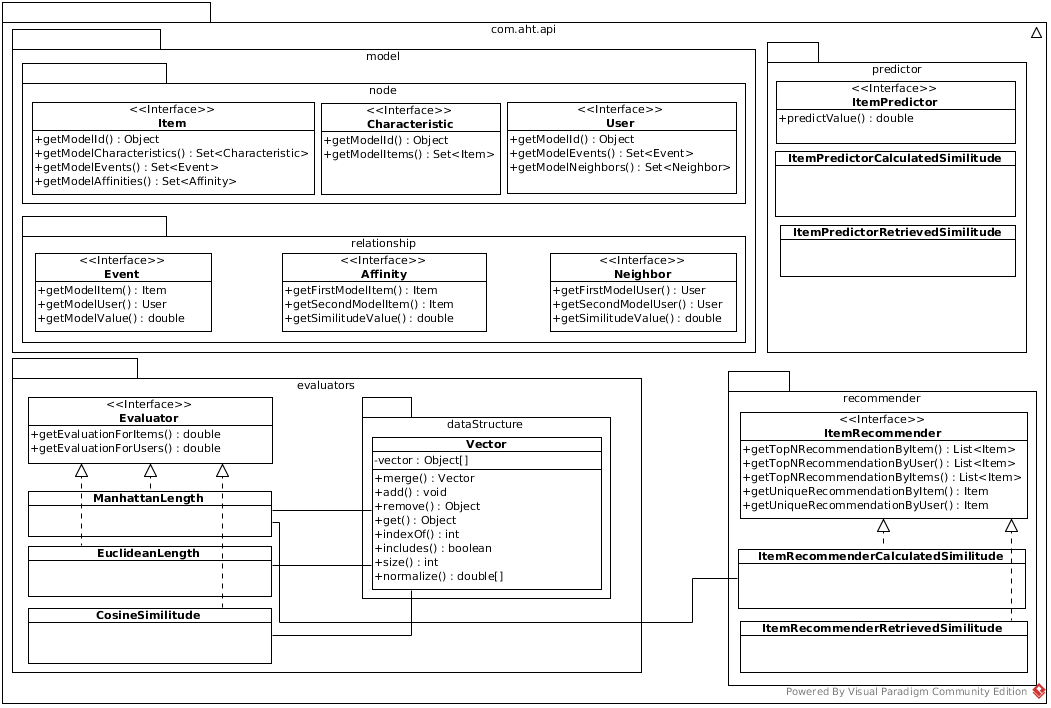
\includegraphics[width=24cm]{./images/classes_api}
      \caption{Diagrama de clases de la API}
      \label{fig:p3_interfaces}
    \end{figure}
  \end{landscape}

    \begin{figure}[h!]
      \centering
      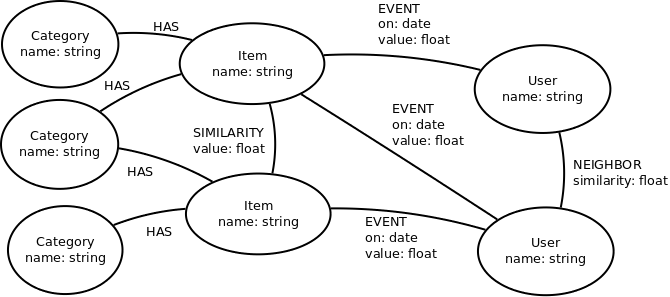
\includegraphics[width=16cm]{./images/general_data_model}
      \caption{Modelo generalizado de datos}
      \label{fig:p3_general_model}
    \end{figure}

  \subsection{Interfaces utilizadas para el modelo de entidades y relaciones}
    \paragraph{Item}
    Describe una entidad de tipo ítem. Estas entidades son el objetivo a recomendar por parte del sistema. Es decir, que el procesamiento lógico tiene como finalidad la recomendación de solo entidades de esta clase.

    \paragraph{User}
    Describe el comportamiento de una entidad de tipo usuario. Estas entidades son responsables de alimentar el sistema a través de su interacción con los artículos a recomendar. Gracias a dichas interacciones es posible obtener información paara generar recomendaciones.

    \paragraph{Characteristic}
    Describe una entidad de tipo característica. Este tipo de entidad permite la abstracción de características propias de las entidades de tipo \emph{Item}  que son determinantes para su categorización. Estas características fungen como un catálogo de los posibles valores existentes entre los diferentes tipos de artículos, gracias a la relación existente entre un \emph{Item} y sus características es posible llevar a cabo la recomendación basada en contenido.

    \paragraph{Event}
    Describe la relación existente entre un usuario y un ítem. Teniendo como propiedad un valor numérico que determina el peso de la relación, ya sea dada por un rating cuantitativo del usuario o por la cantidad de veces que el usuario ha tenido determinada interacción con el ítem.

    \paragraph{Affinity}
    Describe una relación entre dos ítems o artículos. Esta relación tiene como propiedad un valor de similitud determinado por una función de distancia o pseudo-distancia entre los mismos. Como resultado de esto, es posible determinar como objetivo la minimización de distancia o bien la maximización de similitud.

    \paragraph{Neighbor}
    Describe una relación entre dos usuarios registrados del sistema. Dicha relación se ve determinada por las interacciones entre usuarios e ítems, estas interacciones determinadas por los eventos de un usuario permiten a través del procesamiento de los datos, calcular una distancia o pseudo-distancia entre él y otros usuarios registrados, resultando en el valor para dicha relación. 

    Las interfaces descritas previamente permiten como resultado la manipulación de los datos de manera generalizada. 

  \subsection{Interfaces utilizadas para la recomendación y posible extensión de funcionalidad}
    Para realizar las recomendaciones, fue necesario tener diferentes servicios determinados por funciones de recomendación, de predicción y evaluadores para obtener las distancias o pseudo-distancias a utilizar. Para esto se planteó el uso de las interfaces \emph{ItemRecommender}, \emph{ItemPredictor} y \emph{Evaluator}.

    \paragraph{\emph{ItemRecommender}}
      Describe el comportamiento de la implementación de un algoritmo de recomendación que tiene como objetivo devolver un conjunto de ítems que representan una recomendación. Ejemplo de implementaciones son las clases \emph{ItemRecommenderGeneral} y \emph{ItemRecommenderNeo4j} las cuales describen la implementación de algoritmos para filtrado por contenido y filtrado colaborativo. \emph{ItemRecommenderGeneral} hace uso del modelo general sin relaciones de afinidad ni vecindad, y por su parte \emph{ItemRecommenderNeo4j} hace uso del modelo general dependiendo del mantenimeinto de las relaciones de afinidad y vecindad. 

    \paragraph{\emph{ItemPredictor}}
      Describe el comportamiento de un predictor de valores para un respectivo ítem o conjunto de ítems y un respectivo usuario. De esta manera, es posible determinar cuantitativamente un valor esperado u aproximado de una inexistente y tal vez futura relación entre un usuario y un ítem. Este valor es determinado por la similitud existente entre el ítem evaluado y el conjunto de ítems con los que un usuario ha interactuado previamente. Ejemplos de implementaciones se desarrollaron en \emph{ItemPredictorGeneral} e \emph{ItemPredictorNeo4j} 

    \paragraph{\emph{Evaluator}}
      Esta interfaz describe el comportamiento de las funciones de evaluación necesarias para calcular la distancia o pseudo-distancia entre dos items o usuarios. Este valor describe la diferencia o similitud con base en la distancia calculada, dependiendo del algoritmo de evaluación implementado. Ejemplo de clases que implementan esta interfaz son \emph{ManhattanLenght}, \emph{EuclideanLength} y \emph{CosineSimilitude}. 

    
  \section{Resultados}
    Para comprobar las funcionalidades de la API, se utilizaron las clases de dominio Dish, Characteristic y User las cuales implementan las interfaces de modelo para las entidades, descritas con anterioridad.

    Así mismo, se utlizaron las clases Affinity y Neighbor implementando las interfaces de modelo para las relaciones. Estas clases de dominio mapean los resultados del modelo de datos que se puede observar en la figura~\ref{fig:p3_db}

    \begin{figure}[h!]
      \centering
      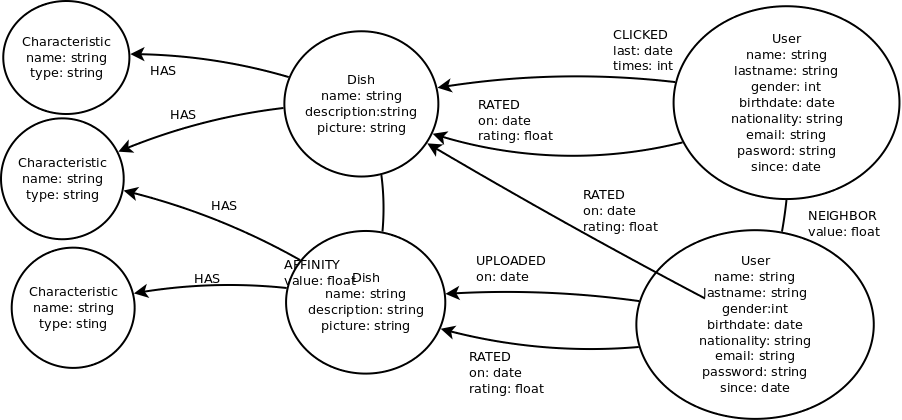
\includegraphics[width=16cm]{./images/p3_bd}
      \caption{Modelo de datos para el prototipo 3}
      \label{fig:p3_db}
    \end{figure}

    Utilizando las interfaces propuestas en la API, se crean las clases de dominio Dish, User y Characteristic para las entidades, así como Rate, Affinity y Neighbor para el modelado de las relaciones como se muestra en la figura~\ref{fig:p3_classes}

  \begin{landscape}
    \begin{figure}[h!]
      \centering
      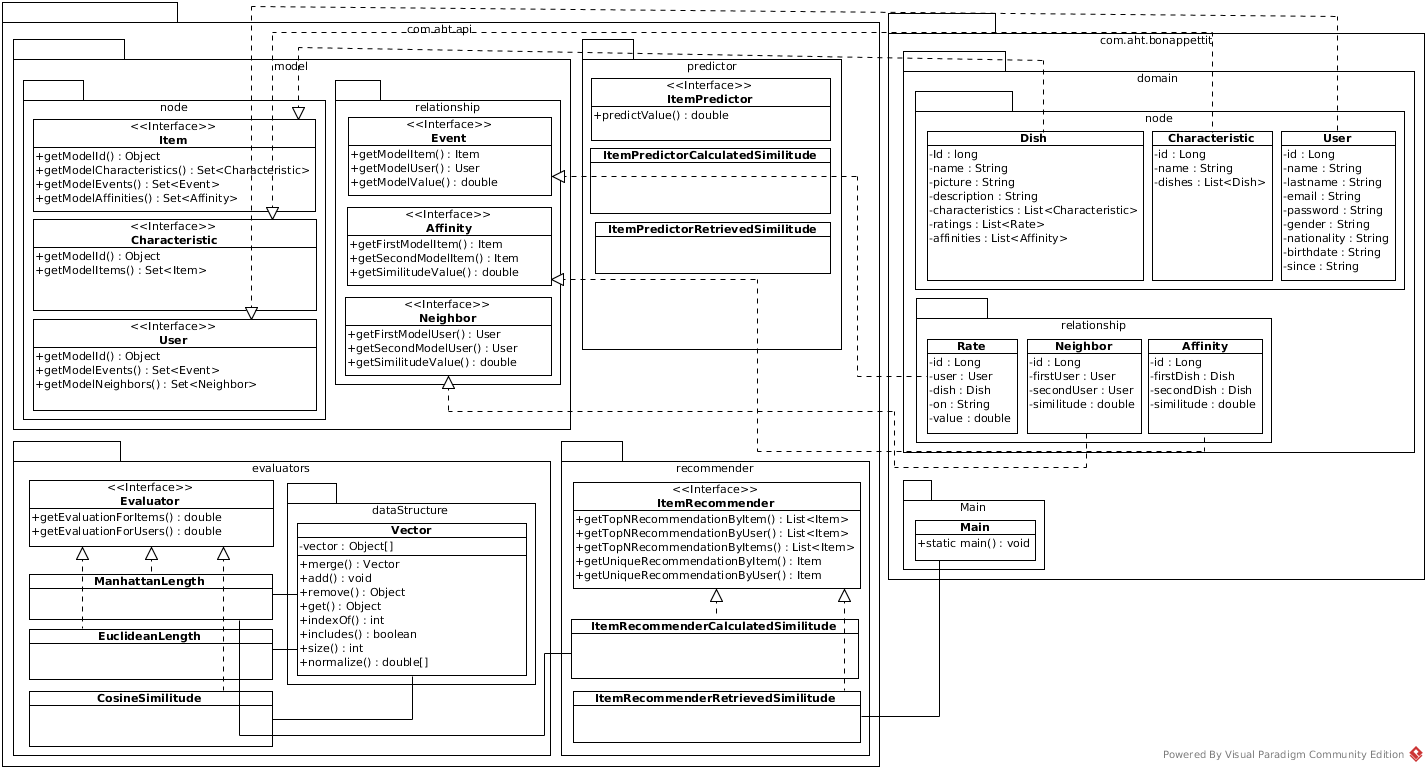
\includegraphics[width=25cm]{./images/p3_classes}
      \caption{Diagrama de clases del prototipo 3}
      \label{fig:p3_classes}
    \end{figure}
  \end{landscape}




  \chapter{Prototipo 4: Desarrollo de un sistema híbrido de recomendación de platillos}
  \section{Análisis}
    \subsection{Objetivo}
      Desarrollar un sistema híbrido para la recomendación de platillos que conlleve la demostración de la funcionalidad proporcionada por el API en un caso de estudio particular.

    \subsection{Características}
    \begin{itemize}
      \item El sistema permitirá realizar recomendaciones de platillos de acuerdo a sus características de los mismos (basadas en contenido).
      \item El sistema permitirá realizar recomendaciones de platillos con base en la interacción de los usuarios finales a través de ratings o evaluaciones cuantitativas (por filtrado colaborativo).
      \item El sistema permitirá el registro de usuarios finales, así como su autenticación para el uso de las funcionalidades del sistema.
      \item El sistema permitirá la visualización de los platillos a los usuarios no registrados.
      \item El sistema permitirá la recomendación para los usuarios no registrados a través del manejo de cookies en el navegdor y su interacción con los platillos.
    \end{itemize}

    \subsection{Restricciones}
    \begin{itemize}
      \item El sistema se verá limitado a las características y cantidad de platillos registrados para realizar las recomendaciones.
      \item El sistema no permitirá el registro de platillos a usuarios no registrados.
    \end{itemize}

    % Insertar historias de usuario aqui

  \section{Diseño}

    Para desarrollar las características mencionadas previamente, se debe tomar en cuenta el modelo de datos propio del caso de estudio que podemos observar en la figura ~\ref{fig:model_cs}

    \begin{landscape}
      \begin{figure}[h!]
        \centering
        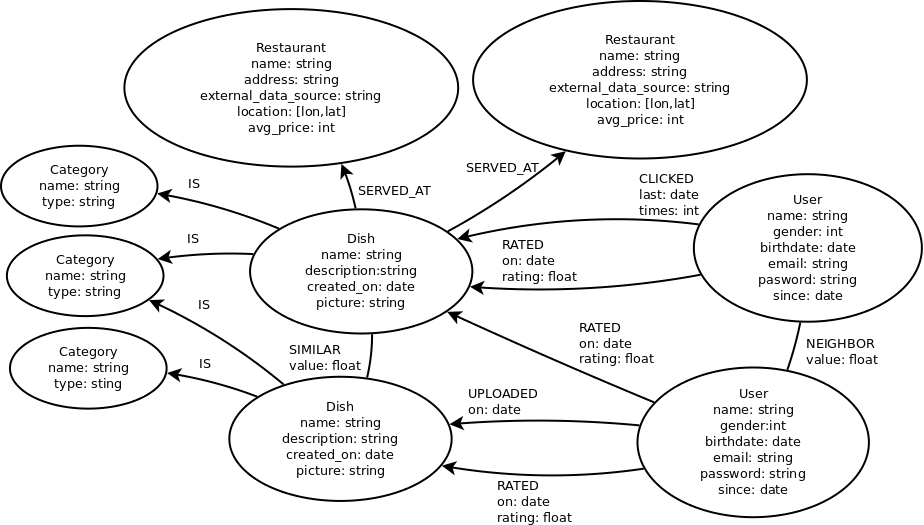
\includegraphics[width=25cm]{./images/sc_data_model}
        \caption{Modelo de datos del caso de estudio}
        \label{fig:model_cs}
      \end{figure}
    \end{landscape}

  Web Services
  Se desarrollaron un conjunto de clases para exponer las operaciones básicas de un CRUD de las clases de dominio User, Dish, Category y Restaurant así como para la creación de las relaciones entre estas entidades.

  Estas clases se componen de tres partes importantes: un recurso que identificará a cada una de estas clases, para este caso, se decidió poner el nombre de la entidad a la que hacen referencia y concatenando la palabra ws; la segunda es el nombre del recurso que identificará a cada uno de los métodos de esta clase. Cada uno de estos métodos son POST. Al crear los métodos de esta clase para que manipulara las cinco operaciones del CRUD 
  (Creat, Retrieve, Update, Delete y RetrieveAll) se decidió utilizar el mismo nombre. Por último, se debe declarar el tipo de respuesta que tienen estos métodos. Para cada uno de ellos se regresa una respuesta que contiene un JSON; cada uno de los JSON posee un campo llamado succes, el cual actua como una bandera para indicar si la operacion fue éxitosa o no.

  \section{Resultados}
    Utilizando el comportamiento de la API como parte de la funcionalidad del sistema, integrado con las clases de dominio y los servicios diseñados previamente obtenemos la estructura mostrada en el diagrama de clases de la figura~\ref{fig:monster_classes}. 

    \begin{landscape}
      \begin{figure}[h!]
        \centering
        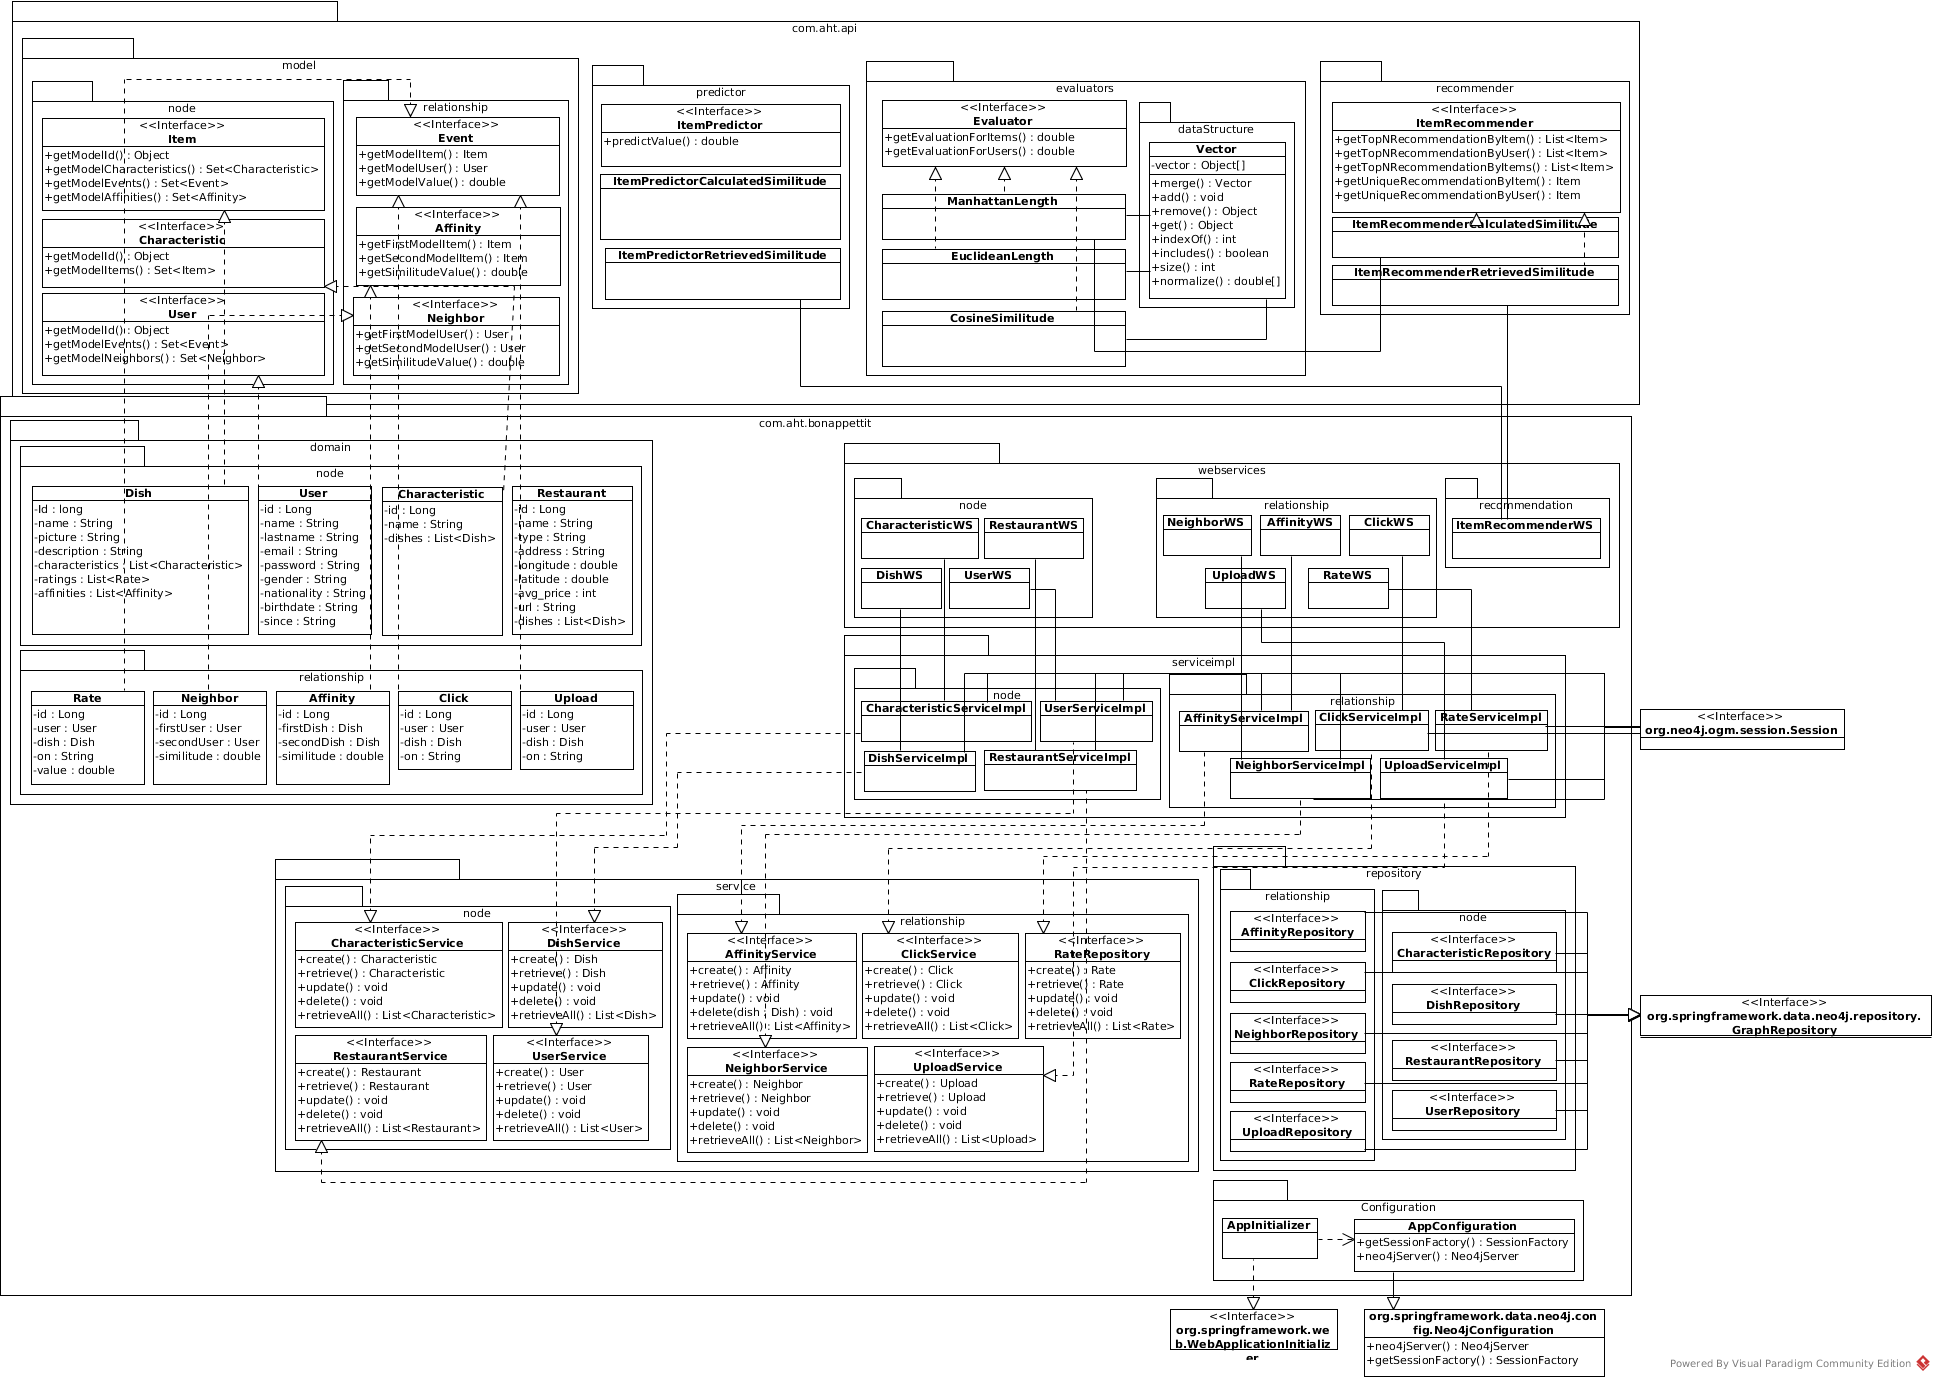
\includegraphics[width=25cm]{./images/monster_class}
        \caption{Diagrama de clases del prototipo 4}
        \label{fig:monster_classes}
      \end{figure}
    \end{landscape}

    Así finalmente podemos desarrollar el sistema, consumiendo los servicios web proporcionados por el back-end del sistema en una aplicación de angular, que a través de servicios y controladores que siguen el patrón MVC, permiten mostrar los datos en una interfaz gráfica al usuario final, como la mostrada en la figura~\ref{fig:final_bonappettit}


      \begin{figure}[h!]
        \centering
        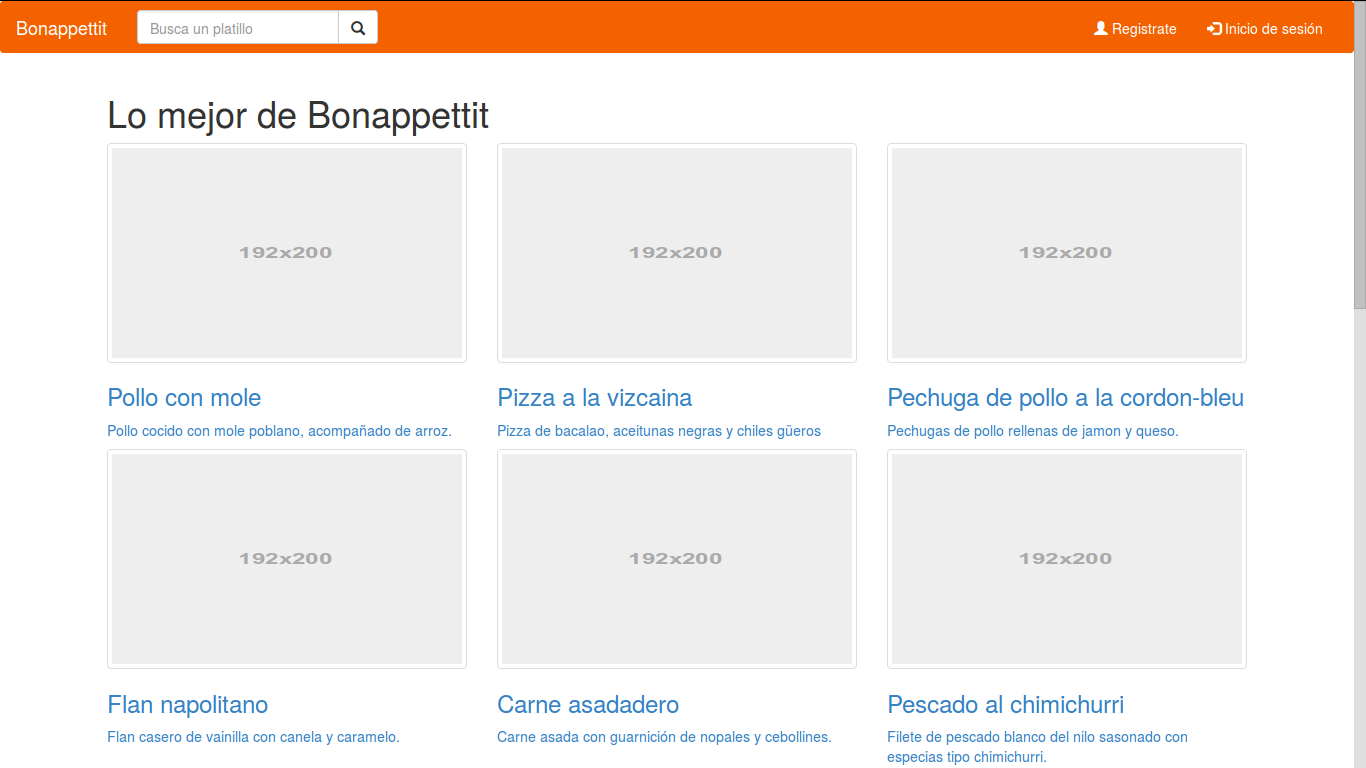
\includegraphics[width=16cm]{./images/p4_bonappettit}
        \caption{Interfaz gráfica del sistema}
        \label{fig:final_bonappettit}
      \end{figure}


  \newpage
\chapter{Anexos}

\iffalse
\newpage
\section*{Pruebas unitarias}
\subsection*{Smart Owl}
\begin{center}
  \includegraphics[width=\textwidth]{images/SmartOwlTest1}
\end{center}

\begin{center}
  \includegraphics[width=\textwidth]{images/SmartOwlTest2}
\end{center}

\begin{center}
  \includegraphics[width=\textwidth]{images/SmartOwlTest3}
\end{center}
\addcontentsline{toc}{chapter}{Anexo 1: Pruebas Unitarias}
%
% User stories
%
\newpage
\section*{Historias de Usuario}
\subsection*{Friendly Dolphin}
  \begin{itemize}
    \item US1 Reporte de información climática actual
    \begin{itemize}
      \item \textbf{Como} usuario de Friendly Dolphin
      \item \textbf{Quiero} consultar la información climática actual
      \item \textbf{De tal manera} que pueda generar un reporte con la información estandarizada.
    \end{itemize}
    \item Criterios de Aceptación
    \begin{itemize}
      \item Seleccionar una región del pais.
      \item Se deberá mostrar la información en texto plano.
      \item Opción para exportar la información en formato JSON o XML.
    \end{itemize}
  \end{itemize}
  \begin{itemize}
    \item US2 Historial de información climática
    \begin{itemize}
      \item \textbf{Como} usuario de Friendly Dolphin
      \item \textbf{Quiero} consultar el historial de los datos climáticos.
      \item \textbf{De tal manera} que pueda visualizar de manera gráfica el cambio de los valores de las variables climáticas a través de un periodo de tiempo
    \end{itemize}
    \item Criterios de Aceptación
    \begin{itemize}
      \item Consultar la información entre una fecha de Inicio y una fecha Final.
      \item Se deberá mostrar la información de las variables climáticas en el periodo seleccionado.
      \item Opción para exportar la información en formato JSON o XML.
    \end{itemize}
  \end{itemize}
\addcontentsline{toc}{chapter}{Anexo 2: Historias de Usuario.}
%
% RESTful Services
%
\newpage
\section*{Servicios REST}
\paragraph{La ventaja al usar servicios de tipo REST, es la sencillez al cambiar el contenido que se expone sin tener que cambiar o generar un protocolo de comunicación ya que toma como base HTTP}.
\paragraph{Simplemente es necesario con un cliente, desde un navegador web hasta clientes dedicados a servicios REST, para poder accedera a los recursos expuestos. Todas las API's rest siguen una convención de verbos tomados de la base de HTTP (GET, POST, PUT, DELETE).}
\paragraph{En comparación con servicios de tipo SOAP, no se requiere una alta atomicidad y ni transacciones, una de las razones por la que los servicios WS suelen ser usados.}
\paragraph{Finalmente, los servicios de tipo REST pueden tener respuestas en diversos formatos, principalmente JSON y XML, esto brinda al desarollador o a la persona que consula como tratar la respuesta por bibliotecas de terceros o nativas.}
\paragraph{El soporte para formatos JSON es nativo en los navegadores web, otra de las razones por las cuales éstos servicios han ido ganando mercado ya que el desarrollo de aplicaciones Web ha aumentado de forma drástica en los últimos años. \cite{31}}
\addcontentsline{toc}{chapter}{Anexo 3: Servicios REST}
\fi
\section{Categorías propuestas para el caso de estudio}
  \begin{table}[h]
    \begin{center}
      \begin{tabular}{ | c | c | c | c | c | c |}
        \toprule
        Id & Tipo & Categoría & Id & Tipo & Categoría\\
        \midrule
        1 & kind  & Panes y masas & 47 & occasion  & Ocasión especial \\
        \midrule
        2 & kind  & Pastas & 48 & region  & Italiana \\
        \midrule
        3 & kind  & Bizcochos y galletas & 49 & region  & Mediterránea \\
        \midrule
        4 & kind  & Carnes & 50 & region  & Asiática \\
        \midrule
        5 & kind  & Aves & 51 & region  & Mexicana \\
        \midrule
        6 & kind  & Pescados y mariscos & 52 & region  & Americana \\
        \midrule
        7 & kind  & Ensaladas & 53 & region  & Hindú \\
        \midrule
        8 & kind  & Contenido alcohólico & 54 & region  & Francesa \\
        \midrule
        9 & kind  & Salsas y guarniciones & 55 & region  & Tailandesa \\
        \midrule
        10 & kind  & Sopas y cremas & 56 & region  & Cantonesa \\
        \midrule
        11 & kind  & Arroces & 57 & region  & Japonesa \\
        \midrule
        12 & kind  & Legumbres y guisos & 58 & region  & China \\
        \midrule
        13 & kind  & Tartas y dulces & 59 & region  & Medio oriente \\
        \midrule
        14 & kind  & Helados y sorbetes & 60 & region  & Alemana \\
        \midrule
        15 & kind  & Frutas & 61 & region  & Argentina \\
        \midrule
        16 & kind  & Verduras & 62 & region  & Brasileña \\
        \midrule
        17 & kind  & Huevos & 63 & region  & Colombiana \\
        \midrule
        18 & kind  & Lácteos & 64 & region  & Coreana \\
        \midrule
        19 & kind  & Frutos secos & 65 & region  & Cubana \\
        \midrule
        20 & kind  & Encurtidos y conservas & 66 & region  & Española \\
        \bottomrule
      \end{tabular}
    \end{center}
  \end{table}
  \begin{table}
    \begin{center}
      \begin{tabular}{ | c | c | c | c | c | c |}
        \toprule
        Id & Tipo & Categoría & Id & Tipo & Categoría\\
        \midrule
        21 & kind  & Postre & 67 & region  & Finlandesa \\
        \midrule
        22 & kind  & Bebida & 68 & region  & Griega \\
        \midrule
        23 & kind  & Primeros platos & 69 & region  & Holandesa \\
        \midrule
        24 & kind  & Segundos platos & 70 & region  & Indonesa \\
        \midrule
        25 & kind  & Entradas & 71 & region  & Portuguesa \\
        \midrule
        26 & kind  & Sopas y cremas & 72 & health  & Bajas en colesterol \\
        \midrule
        27 & kind  & Acompañamientos & 73 & health  & Diabéticos \\
        \midrule
        28 & kind  & Emparedados & 74 & health  & Sin lactosa \\
        \midrule
        29 & kind  & Botana & 75 & health  & Celiacos \\
        \midrule
        30 & kind  & Comida rápida & 76 & health  & Alérgicos \\
        \midrule
        31 & flavour  & Dulce & 77 & health  & Bajar de peso \\
        \midrule
        32 & flavour  & Salado & 78 & health  & Vegetarianos \\
        \midrule
        33 & flavour  & Ácido & 79 & temperature  & Frío \\
        \midrule
        34 & flavour  & Amargo & 80 & temperature  & Templado \\
        \midrule
        35 & flavour  & Umami & 81 & temperature  & Caliente \\
        \midrule
        36 & flavour  & Picante & 82 & people  & Bebes \\
        \midrule
        37 & occasion  & Halloween & 83 & people  & Niños \\
        \midrule
        38 & occasion  & Navidad & 84 & people  & Adultos \\
        \midrule
        39 & occasion  & San Valentín & 85 & people  & Familiares \\
        \midrule
        40 & occasion  & Primavera & 86 & people  & Adultos mayores \\
        \midrule
        41 & occasion  & Verano & 87 & texture  & Liquidas \\
        \midrule
        42 & occasion  & Otoño & 88 & texture  & Blandas \\
        \midrule
        43 & occasion  & Invierno & 89 & texture  & Semi-blandas \\
        \midrule
        44 & occasion  & Desayunos & 90 & texture  & Crujientes \\
        \midrule
        45 & occasion  & Almuerzos & 91 & texture  & Duras \\
        \midrule
        46 & occasion  & Meriendas & & & \\
        \bottomrule
      \end{tabular}
      \caption{Categorías propuestas para el caso de estudio}
      \label{Categorías propuestas para el caso de estudio}
    \end{center}
  \end{table}
  \newpage
\section*{Glosario}
\begin{itemize}
  \item \textbf{API}: Application Programming Interface, conjunto de rutinas, protocolos o herramientas para construcción de software.
  \item \textbf{ACID:} Es un acrónimo de Atomicity, Consistency, Isolation and Durability: Atomicidad, Consistencia, Aislamiento y Durabilidad en español.
  \item \textbf{Atomicidad:}Si una operación consiste en una serie de pasos, todos ellos ocurren o ninguno, es decir, las transacciones son completas.
  
  \item \textbf{Atributo}: Los atributos son las características individuales que diferencian un objeto de otro y determinan su apariencia, estado u otras cualidades.Los atributos se guardan en variables denominadas de instancia, y cada objeto particular puede tener valores distintos para estas variables.
  \item \textbf{Aislamiento:} es la propiedad que asegura que una operación no puede afectar a otras. Esto asegura que la realización de dos transacciones sobre la misma información sean independientes y no generen ningún tipo de error.  Esta propiedad define cómo y cuándo los cambios producidos por una operación se hacen visibles para las demás operaciones concurrentes.
  \item \textbf{Base De Datos:} Es un conjunto de datos pertenecientes a un mismo contexto y almacenados sistemáticamente para su posterior uso.
  \item  \textbf{Caso De Uso:} Es una descripción de los pasos o las actividades que deberán realizarse para llevar a cabo algún proceso. 
  \item \textbf{Consistencia:} Es la propiedad que asegura que sólo se empieza aquello que se puede acabar. Por lo tanto se ejecutan aquellas operaciones que no van a romper las reglas y directrices de Integridad de la base de datos. La propiedad de consistencia sostiene que cualquier transacción llevará a la base de datos desde un estado válido a otro también válido. 
  \item \textbf{Durabilidad:} Persistencia. Es la propiedad que asegura que una vez realizada la operación, ésta persistirá y no se podrá deshacer aunque falle el sistema y que de esta forma los datos sobrevivan de alguna manera.
  \item \textbf{Entidad:} Representa una cosa u objeto del mundo real con existencia independiente, es decir, se diferencia únicamente de otro objeto o cosa, incluso siendo del mismo tipo, o una misma entidad.
  \item \textbf{Framework: }Es una estructura conceptual y tecnológica de soporte definido, normalmente con artefactos o módulos concretos de software, que puede servir de base para la organización y desarrollo de software. 
   \item \textbf{Grafo:} Estructura la información en forma de nodos y relaciones.
   \item \textbf{Prototipo:} Es una representación de un sistema, aunque no es un sistema completo, posee las características del sistema final o parte de ellas.
   \item \textbf{Recomendación:} Conjunto de objetos que por sus características determinan ser relevantes para un usuario. 
   \item \textbf{Web Scrapping:} Técnica implemendatada mediante programas de software para extraer información de sitios web.
    \item \textbf{Cold Start:} Sistema que carece de datos para producir recomendaciones.
\end{itemize}
\addcontentsline{toc}{chapter}{Glosario}
  \begin{thebibliography}{99}
  %Introduction
  \bibitem{1}
    Roger Loaiza. \emph{¿Qué es la inteligencia artificial?. “De la información a la informática”}. Obtenido desde \url{http://bvs.sld.cu/revistas/san/vol2_2_98/san15298.htm} el 1 de mayo de 2015.
  \bibitem{2}
    Enrique Herrera-Viedma, \emph{Sistemas de recomendaciones: herramientas para el filtrado de información en Internet}, 2004. Obtenido desde \url{http://www.upf.edu/hipertextnet/numero-2/recomendacion.html} el 2 de mayo de 2015. 
  \bibitem{3}
     Marcos Merino. \emph{¿Qué es una API y para qué sirve?} Obtenido desde: \url{http://www.ticbeat.com/tecnologias/que-es-una-api-para-que-sirve/} el 4 de mayo de 2015. 

  %Background
  \bibitem{4}
    Paul Resnick and Hal R. Varian, Recommender Systems. 1997. Obtenido desde: \url{https://www.ischool.utexas.edu/~i385d/readings/Resnick_Recommender_97.pdf}
  \bibitem{5}
    Robin Burke, California State University, Fullerton \emph{Hybrid Recommender Systems: Survey and Experiments}. Obtenido desde: \url{http://citeseerx.ist.psu.edu/viewdoc/download?doi=10.1.1.88.8200\&rep=rep1\&type=pdf}
  \bibitem{6}
    Gediminas Adomavicius, Alexander Tuzhilin. \emph{Towards the Next Generation of Recommender Systems: A Survey of the State-of-the-Art and Possible Extensions}. Obtenido desde: \url{http://homepages.dcc.ufmg.br/~nivio/cursos/ri13/sources/recommender-systems-survey-2005.pdf}
  \bibitem{7}
    Chad Vicknair, Michael Macias, Zhendong Zhao, Xiaofei Nan, Yixin Chen, Dawn Wilkins. \emph{A Comparison of a Graph Database and a Relational Database}. Obtenido desde: \url{http://cs.olemiss.edu/~ychen/publications/conference/vicknair_acmse10.pdf}
  \bibitem{8}
    Renzo Angles , Claudio Gutierrez. \emph{Survey of Graph Database Models} Obtenido desde: \url{http://www.dcc.uchile.cl/TR/2005/TR_DCC-2005-010.pdf}
  \bibitem{9}
    Bases de Datos Orientadas a Grafos. Obtendo desde \url{http://www.bigdatahispano.org/noticias/bases-de-datos-orientadas-a-grafos/} 
  \bibitem{10}
    Brian Proffitt, \emph{What APIs Are And Why They're Important}. Sep 19, 2013. Obtenido desde: \url{http://readwrite.com/2013/09/19/api-defined}
  \bibitem{11}
    Sofía Marina Pepa, \emph{Suite de algoritmos de recomendación en aplicaciones reales}. Obtenido desde: \url{https://repositorio.uam.es/bitstream/handle/10486/660903/marina_pepa_sofia_tfg.pdf?sequence=1}

  %Related Work
  \bibitem{12}
     Spotify. Obtenido desde: \url{https://www.spotify.com/mx/about-us/contact/}
  \bibitem{13}
     Sistema Generador de Recomendaciones para una Tienda En-Línea de Videojuegos, 2010. ESCOM IPN. 
  \bibitem{14}
    Gregory Piatetsky. Prediction.io open source machine learning server, 10 de abril de 2014. Obtenido desde: \url{http://www.kdnuggets.com/2014/04/prediction-io-open-source-machine-learning-server.html} el 6 de mago de 2015. 
  \bibitem{15}
    Easyrec, Obtenido desde \url{http://easyrec.org/} el 6 de mayo de 2015 
  \bibitem{16}
    REST API. Obtenido desde: \url{http://easyrec.sourceforge.net/wiki/index.php?title=REST_API_v0.98} el 6 de mayo de 2015. 
  \bibitem{17}
    Netflix. Obtenido desde: \url{https://help.netflix.com/es/node/412} 6 de mayo de 2015.
  \bibitem{18}
    Lenskit: Open-Source Tools for Recommender Systems. Obtendo desde \url{http://lenskit.org/}

  %Technologies
  \bibitem{19}
    Neo4j Obtendo desde \url{http://xurxodeveloper.blogspot.mx/2014/03/neo4j-una-base-de-datos-nosql-orientada.html/}
  \bibitem{20}
    Cómo Funciona Neo4j Obtendo desde \url{http://bbvaopen4u.com/es/actualidad/neo4j-que-es-y-para-que-sirve-una-base-de-datos-orientada-grafos/}
  \bibitem{21}
    Neo4j-Rendimiento Obtendo desde \url{http://bbvaopen4u.com/es/actualidad/neo4j-que-es-y-para-que-sirve-una-base-de-datos-orientada-grafos/}	
  \bibitem{22}
    Oracle y Java, características. Obtenido desde \url{http://www.oracle.com/es/technologies/java/features/index.html}

  %Prototype 1
  \bibitem{23}
      Alergia a los alimentos. Obtenido desde: \url{http://www.laalergia.com/tipos-alergia/alimentos/}
  \bibitem{24}
      ReceTags: Recetario en línea. Obtenido desde: \url{http://www.recetags.com/}

     \bibitem{27}
   Tipos de API. Obtenido desde \url{http://www-01.ibm.com/support/knowledgecenter/SS6PEW_9.4.0/com.ibm.help.custom.apis.doc/API_API_Types.html?lang=es}
   	\bibitem{28}
   Bases de datos relacionales. Obtenido desde J. J. King, «QUIST: A System for Semantic Query Optimization in Relational Data Bases», Proc. of the International Conf. on Very Large Databases (1981),
páginas 510-517
   \bibitem{29}
   Bases de datos no relacionales. Obtenido desde \url{ «NoSQL Relational Database Management System: Home Page». Strozzi.it. 2 de octubre de 2007. Consultado el 10 de Noviembre de 2015.}
   \bibitem{30}
   Bases de datos orientadas a grafos. Obtenido desde \url{ http://graphbase.net/}
   \bibitem{31}
   Bases de datos orientadas a grafos. Obtenido desde \url{ http://xurxodeveloper.blogspot.mx/2014/03/neo4j-una-base-de-datos-nosql-orientada.html}
   \bibitem{32}
   InfiniteGraph. Obtenido desde  Joyce Wells (June 26, 2013). "DBTA 100: The Companies That Matter Most in Data". Database Trends and Applications. Retrieved September 8, 2014.
   \bibitem{33}
   Infogrid. Obtenido desde  \url{http://infogrid.org/trac/}
   \bibitem{34}
   Bootstrap. Obtenido desde  \url{http://getbootstrap.com/2.3.2/}
   \bibitem{35}
   Foundation. Obtenido desde  \url{http://foundation.zurb.com/}
   \bibitem{36}
   Maven. Obtenido desde  \url{http://chuwiki.chuidiang.org/index.php?title=Categor%C3%ADa:Maven}
   \bibitem{37}
   Ant. Obtenido desde  \url{http://ant.apache.org/}
   \bibitem{38}
   Git. Obtenido desde  \url{https://git-scm.com/}
   \bibitem{39}
   Subversion \url{http://svnbook.red-bean.com/nightly/es/svn-ch-1-sect-1.html}
   \bibitem{40}
   Java \url{http://www.oracle.com/technetwork/java/index.html}

\end{thebibliography}


\addcontentsline{toc}{chapter}{Bibliografía}

\end{document}
